\documentclass[stu,12pt,floatsintext,donotrepeattitle]{apa7}
\usepackage{csquotes}
\usepackage{amsmath}
\usepackage[style=apa,sortcites=true,sorting=nyt,backend=biber]{biblatex}
\DeclareLanguageMapping{american}{american-apa}
\addbibresource{MyBib.bib}

% --- FONT CONFIGURATION (ARIAL) ---
\usepackage[T1]{fontenc}
\usepackage{helvet} % Helvet is the standard LaTeX clone for Arial
\renewcommand{\familydefault}{\sfdefault} % Force entire document to use Sans-Serif (Arial)
% \usepackage{mathptmx} % REMOVED: This was forcing Times New Roman

% --- MARGIN CONFIGURATION ---
% apa7 loads geometry automatically, so we overwrite the settings here
\geometry{left=38mm, right=28mm, top=28mm, bottom=28mm}

% --- SPACING AND INDENTATION ---
\usepackage{setspace}
\onehalfspacing % 1.5 Line spacing for text
\usepackage{indentfirst} % Ensure first paragraph of sections is indented
\setlength{\parindent}{12.7mm} % Paragraph indent 12.7mm
\setlength{\parskip}{\baselineskip} % Double spacing between paragraphs

% --- CAPTION CONFIGURATION ---
% Ensures captions for Tables and Charts (Figures) are single spaced
\usepackage[font={singlespacing}]{caption}
\counterwithin{figure}{section}

% --- HEADINGS CONFIGURATION ---
% We use titlesec to override apa7's default section styling
\usepackage{titlesec}
\setcounter{secnumdepth}{3} % Enable numbering (1, 1.1, 1.1.1) which apa7 usually hides

% --- TABLE SPACING ---
% Ensure tables are single spaced per guidelines
\AtBeginEnvironment{tabular}{\singlespacing}
\AtBeginEnvironment{tabularx}{\singlespacing}

\newcommand\nd{\textsuperscript{nd}\xspace}

% Section (Mapped to Chapter Heading): Arial 14pt Bold
\titleformat{\section}
  {\normalfont\sffamily\fontsize{14}{17}\bfseries}{\thesection}{1em}{}
\titlespacing*{\section}{0pt}{0pt}{20pt}

% Subsection (Mapped to Sub-heading): Arial 12pt Bold
\titleformat{\subsection}
  {\normalfont\sffamily\fontsize{12}{14.4}\bfseries}{\thesubsection}{1em}{}

% Subsubsection (Mapped to Sub-sub-heading): Arial 12pt Bold
\titleformat{\subsubsection}
  {\normalfont\sffamily\fontsize{12}{14.4}\bfseries}{\thesubsubsection}{1em}{}


% --- PAGE NUMBERING (Bottom Center) ---
\usepackage{fancyhdr}
\pagestyle{fancy}
\fancyhf{} % Clear default apa7 headers/footers
\fancyfoot[C]{\thepage} % Center footer page number
\renewcommand{\headrulewidth}{0pt} % Remove header line

% Ensure plain pages (like title page) also use this style
\fancypagestyle{plain}{
  \fancyhf{}
  \fancyfoot[C]{\thepage}
  \renewcommand{\headrulewidth}{0pt}
}

% --- PACKAGES ---
\usepackage{enumerate}
\usepackage{enumitem}
\usepackage{xspace}
\usepackage{graphicx}
\usepackage{float}
\usepackage{tabularx}
\usepackage{booktabs}
\usepackage{multirow} 
\usepackage{lipsum}
\usepackage{etoolbox} 
\usepackage{longtable}
\usepackage{pdflscape}

% --- CODE SNIPPET CONFIGURATION ---
\usepackage{listings}
\usepackage{xcolor}

\lstdefinestyle{pythonstyle}{
    backgroundcolor=\color{white},   
    commentstyle=\color{green!50!black},
    keywordstyle=\color{blue},
    stringstyle=\color{purple},
    basicstyle=\ttfamily\footnotesize, % Use a monospaced font
    breakatwhitespace=false,         
    breaklines=true,                 
    captionpos=b,                    
    keepspaces=true,                 
    numbers=left,                    
    numbersep=5pt,
    numberstyle=\tiny\color{gray},
    showspaces=false,                
    showstringspaces=false,
    showtabs=false,                  
    tabsize=2,
    frame=single % Adds a box around the code
}
\lstset{style=pythonstyle}

% --- TABLE SPACING FIX ---
% Ensure tables are single spaced per guidelines
\AtBeginEnvironment{tabular}{\singlespacing}
\AtBeginEnvironment{tabularx}{\singlespacing}

\providecommand{\nd}{}
\renewcommand{\nd}{\textsuperscript{nd}\xspace}
\newcommand\rd{\textsuperscript{rd}\xspace}
\newcommand\nth{\textsuperscript{th}\xspace}

\author{Jordan Ling Shen Hang}
\title{Fake News Detection Using Deep Learning}

\begin{document}
\maketitle

\section{Introduction}

\subsection{Problem Statement}
Fake news threatens personal, organisational and institutions by creating distrust and damaging reputations. Fake news can be particularly damaging as even if it can be refuted, it may still cause lasting damage to reputations. With the widespread use of social media, the proliferation of fake news has greatly increased both in terms of speed and quantity. This has led to the sheer volume of fake news (and real news) overwhelming human fact-checkers and preventing them from manually verifying all content. 

But what is fake news? According to \textcite{definition} the definition of fake news is generally agreed to be either completely or partially false information, with varying levels of agreement for other additional criteria. Such as the intent to deceive, and if only content in a news format should be counted. For the purpose of this research, the working definition of fake news defined by \textcite{definition} will be used: 

\begin{quote}
    a type of online disinformation (1), with (2) misleading
and/or false statements that may or may not be associated with real events, (3) intentionally
created to mislead and/or manipulate a public (4) specific or imagined, (5) through the
appearance of a news format with an opportunistic structure (title, image, content) to attract
the reader’s attention, in order to obtain more clicks and shares and, therefore, greater
advertising revenue and/or ideological gain \textcite{definition}
\end{quote} 

In a recent (as of writing) example of fake news causing adverse impact, \textcite{Savage-Guardian_2025} wrote for The Guardian about YouTube channels spreading fake news about UK politics in their videos, acruing close to 1.2 billion views in total. While some forms of news which are factually fake are usually harmless (parody, satire, etc.) fake news, with the intent or deceiving those who consume it is dangerous, it can widen division, spread prejudice and cause distrust in institutions are among just a few examples. And while fake news may sound innoculous enough, 'It's just fake news, ignore it', it can lead to serious consequnces, including injury and death. In one such example, during the COVID-19 vaccination campaign in Taiwan an adverse correlation between prevalence of fake news and vaccination rates were found \parencite{vaccination}.

As a result, the development of automated fake news detection systems have been explored. But limitations related to generalisation where detection systems perform poorly on data which did not appear in its training sets \parencite{BERT-finetuning} limit their applicability. Additionally, current methods such as Machine Learning (ML) approaches, fail to capture the semantic data meaningfully, reducing its detection accuracy. Furthermore, many approaches which employ Deep Learning (DL) are often black-boxes, which results in lowered trust towards these systems \parencite{xai-bert}. 

This highlights the need for new approaches which are capable of detecting fake news by analysing the semantic information in the text throughly, having greater generalisation and be more transparent (explainable) when making its classifications.

\subsection{Research Objectives}
The objectives of this project are:
\begin{itemize}
    \item Review on methods to detect fake news
    \item Develop a fake news detection using deep learning
    \item Evaluate the performance of model in detection fake news
\end{itemize}

\subsection{Research Scope}
This project aims to build a deep learning model for fake news detection by first conducting a thorough literature review on related works in order to construct a knowledge base of which will be used to construct a model for detecting fake news. \\

After the literature review, a model to detect fake news will be developed using deep learning techniques. This process will involve gathering datasets, analysing and understanding the data and pre-processing datasets before constructing the architecture of the models and then training the various models. \\ %are we proposing new models?

And lastly, after training the models. The models will be tested on the test sets which are subsets of the datasets used in order to determine their performance.

\begin{figure}[H]
    \centering
    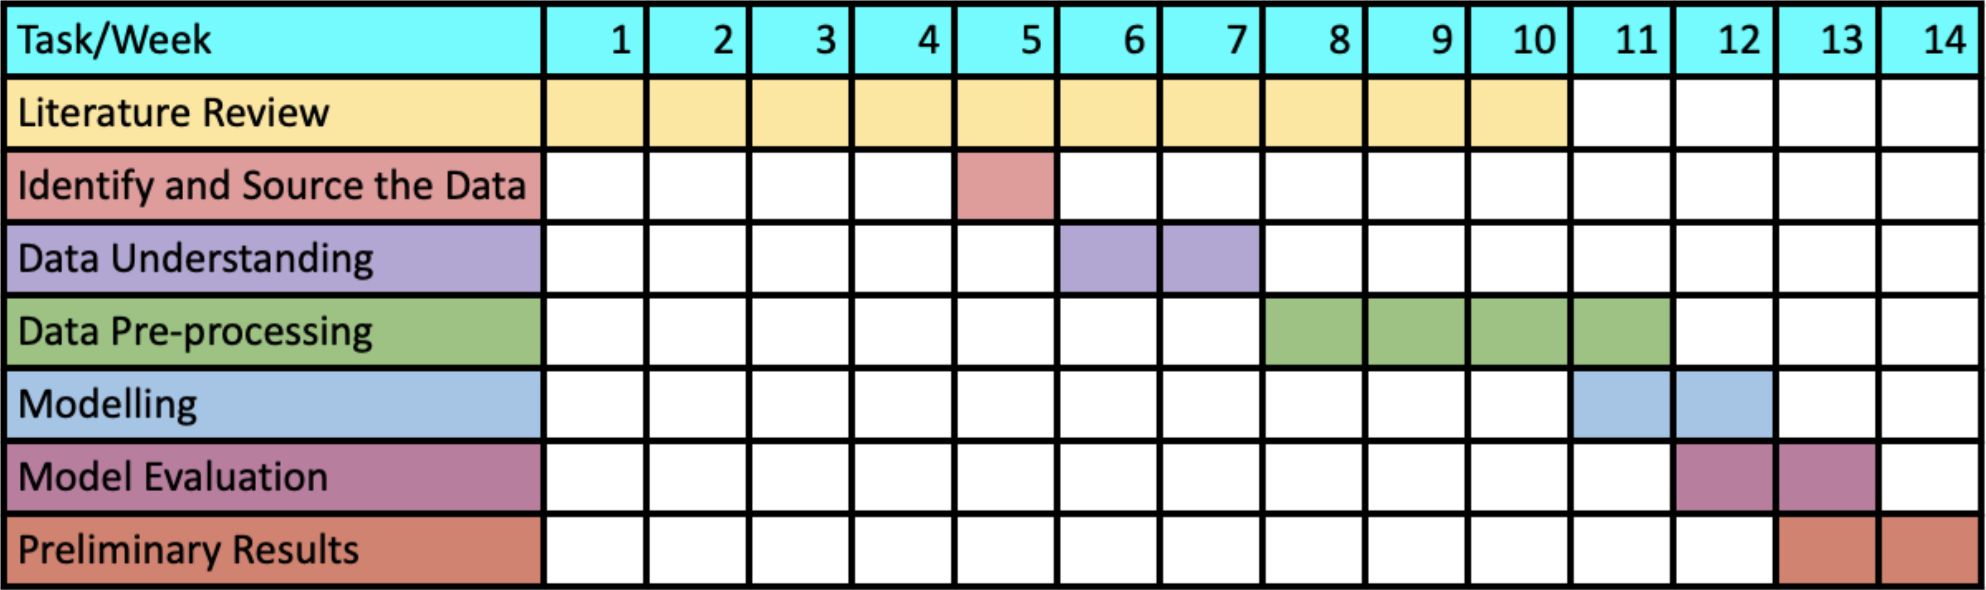
\includegraphics[width=0.8\linewidth]{FYP1-Gantt_chart.png}
    \caption{Gantt chart depicting the timeline for this project relative during MMU's term 2530}
    \label{fig:placeholder}
\end{figure}

\section{Literature Review}
\subsection{Deep Learning Methods and Other Modelling Techniques}
\subsubsection{Convolutional Neural Networks}
In research conducted by \textcite{cnn_chinese}, which detected fake news on Chinese social media networks using an augmented Convolutional Neural Network (CNN), Convolutional Feed-Forward or Conv-FFD. In order to process the Chinese characters, the researchers used a three-step process starting with one-hot-encoding the over 4000 Chinese characters, then feeding this data in an embedding process which converts the one-hot-encoded data into vector representations of each character, culminating in iterating through all the characters to get the vector representation of each one (essentially mapping the characters to the vector embedding). As for the feature modelling process (the process of understanding the relationship between characters/words), the researchers used the CNN model which is able to learn hidden features from conducting convolution operations. They used a 'sliding window' in order to create sentence-level embedding. Then in order to classify the text as real or fake, a softmax activation function is used in order to predict the class of the input text. The model achieved an F1-score of 0.8702 - 0.8855, indicating it is capable of predicting whether a given body of (Chinese) text is real or fake. \\

Research conducted by \textcite{opcnn-fake} also proposed a CNN model, albeit a modified one they called the "optimized Convolutional Neural Network to detect fake news" or OPCNN-FAKE. Aside from the proposed models, the authors also built machine learning models and other deep learning models like LSTMs The authors used four datasets, Fake News Detection (from Kaggle), FakeNewsNet, FA-KES5, and the ISOT dataset. The datasets were cleaned by converting all characters to lowercase, removing URLS, removing special symbols, removing stop words, tokenisation and stemming (reduction to root word). After the data was cleaned, two methodologies were used for feature generation, one for training the machine learning models and one for the deep learning models. For machine learning models, the feature generation used two techniques, N-grams (up to n = 4) and Term Frequency - Inverse Document Frequency (TD-IDF). While for the deep learning models, feature generation was done via word embeddings (the authors classified this as the "Embedding Layer" or the first layer of the proposed OPCNN-FAKE model), specifically the Global Vectors for Word Representations (GLoVe) which converted the cleaned textual data into dense vectors (more specifically they used glove6B.zip). The preprocessed datasets were then split 80-20 into training and test sets respectively and the training set was used to train the machine learning and deep learning models, including the proposed OPCNN-FAKE model. For the deep learning models, a technique called "Hyperopt Optimisation" was used to adapt the various model parameters including epoch, dropout and batch size, among others. The proposed OPCNN-FAKE model was configured with six layers, the embedding layer, dropout layer, convolutional layer, pooling layer, flatten layer and output layer respectively. Without diving too deeply into the architecture, the embedding layer was previously explained; the dropout layer randomly deactivates some neurons to mitigate overfitting; the convolutional layer uses a convolution filter and feature map to identify the data patterns and high and low level features while employing a ReLu activation function; the pooling layer reduces the number of features in the feature map so as to only retain the most important features; the flatten layer flattens the feature map into a one-dimensional array; the output layer takes the one dimensional array from the flatten layer and classifies it as fake (0) or true (1). The models were then evaluated using cross-validation and the OPCNN-FAKE model achieved the best F1-score across all four datasets used, with the proposed model achieving an F1-score of 0.959 on the Kaggle dataset and a perfect F1-score of 0.9999 on the ISOT dataset.



\subsubsection{Hybrid Approaches}
There has also been research that looked into hybrid approaches, \textcite{hybrid_cnn-lstm} proposed a hybrid deep learning model combining Long Short Term Memory (LSTM) and CNN. Using publicly available datasets (WELFake, FakeNewsNet and FakeNewsPrediction), the authors first pre-processed the data using lemmatisation (reduction of words to root form), de-capitalisation, tokenisation, among others. To process the cleaned data, the authors used FastText, both its supervised and unsupervised forms to create word embeddings. These words embeddings, generated from both the unspervised and supervised FastText models were then used to train separate models, including ensemble (stacked) machine learning models, transformer models and the CNN-LSTM hybrid mentioned earlier. Evaluation of the models using test subsets of each of the datasets used showed that those trained on unsupervised FastText embeddings performed worse than those trained on supervised FastText embeddings, with F1-scores between 0.83 - 0.97 with significant variation between the datasets it was tested on. Those trained on supervised FastText embeddings were evaluated on subsets of the datasets used (test sets) and had F1-scores of between 0.91 - 0.99. The CNN-LSTM model performed better than all other models (stacked machine learning models and transformer models), with high F1-scores of between 0.97 and 0.99 across all datasets. \\

While most research seems to have been done on detecting fake news in English, research conducted by \textcite{hybrid2} detected fake news in Arabic. The authors used two datasets, Arabic Fake News Dataset (AFND) and their own dataset scraped from Twitter. The authors explored multiple types of models for detecting fake news including machine learning and common deep learning models but they also proposed a hybrid model called Bidirectional Long Short Term Memory – Bidirectional Gated Recurrent Unit (Bi-LSTM – Bi-GRU). This proposed model is structured sequentially, but it can also deal with information bi-directionally and it attempts to leverage the strengths of Bi-LSTMS and Bi-GRUs. Bi-LSTMs and LSTMs in general are excellent at retaining information and addresses the vanishing gradient problem; while GRUs are able to mamnage shorter dependencies and are computationally efficient. For preprocessing, the authors first cleaned the data by removing all punctuation, unicode characters, names, URLs, stop word removal, tokenisation and other standard techniques. The cleaned data was then features were extracted using both supervised and unsupervised FastText which were then used to train models. The Bi-LSTM – Bi-GRU performed the best among all of the models tested, achieving F1-scores of between 0.98 and 0.99 depending on the dataset. \\

\textcite{gbert} proposed a new deep learning model for predicting fake news called "Generative Bidirectional Encoder Representations from Transformers" or GBERT, a hybrid of Generative Pre-Trained Transformer (GPT) and Bidirection Encoder Representations from Transformers (BERT). The authors used two benchmark Indian datasets: The Indian Fake News Dataset (IFND) and FakeNewsIndia Dataset. The standard cleaning and normalisation of the textual data was applied including: decapitalisation, removal of URLs, names, punctuation stop words, numbers and emojis, and the application of stemming and lemmitisation. Now for the feature extraction the cleaned data is fed into two Large Language Model (LLM) components, BERT and GPT. BERT captures word embeddings, with context from every token inputted and outputs a summary of the context inside the input sequence. While GPT captures the global dependencies and semantic coherence in the input data and outputs the last hidden state of the final token. Finally the output from BERT and GPT (the features) are merged together in a concantenation layer before being passed to the dense layer for the final binary classification using a Sigmoid function. The results showed that the proposed GBERT model performed well, with a F1-score of 0.9623. It is worth noting, however, that XGBoost performed well in terms of accuracy (F1-score was not provided for XGBoost) with a score of 93.42\% while the proposed GBERT model has a score of 95.30\%.

\subsubsection{Deep Ensemble Approaches}
Other than approaches with CNNs, LSTMs and machine learning models, there have also been attempts to construct deep ensemble models composed of deep learning models arranged in an ensemble architecture. Research conducted by \parencite{deep-ensemble} proposed a new approach for detecting fake news, by using Sequential deep learning (SDL) models as the base models in an ensemble stacking architecture with a multilevel perceptron classifier at the top. The authors used two datasets: the LIAR and ISOT datasets. The data from each dataset was preprocessed with tokenisation, lemmatisation among other standard techniques for working with textual data. Unlike with other similar works, the authors chose to do multi-class classification because fake news is usually mixed with true news. For the SDLs they are composed of dense and dropout layers. The ReLu activation function is used in all dense layers except the final output layer where a Sigmoid function was used. The ensemble model was evaluated with the test subset of each dataset used, for the LIAR dataset the model achieved F1-scores in a range from 0.48 to 0.82 for the various classes. As for the ISOT dataset, since the dataset only had two classes (real and fake), the model only had to classify true and false, the binary classification was able to achieve a 1.00 accuracy and f1-score using the 2nd stage classifier. \\


\subsubsection{Machine Learning Approaches}
Research conducted by \parencite{traditional-ml} explored the use of machine learning models such as XGBoost, Support Vector Machine (SVM), Naive Bayes, among others. The authors used the LIAR dataset which they then preprocessed by removing noise such as identification (ID), dots, commas and questions as well as stemming (reduction of a word to root form) and removing any suffixes. They then use Part of Speech (POS) to convert the text into tokens and values. They then extracted features by extracting lexical features such as word count, sections of speech etc. and then used the Term Frequency-Inverse Document Frequency (TD-IDF) vectorizer function from the publicly available library sklearn (also known as scikit-learn) to extract unigram and bigram features. The results showed that the accuracy of the models was limited, especially in comparison to approaches using deep learning with the best performing model being the XGBoost model with an accuracy of 0.73. \\

\subsubsection{Multimodal Approaches}
In research conducted by \textcite{multimodal} the researchers employed a multimodal approach instead of a purely textual approach to detection. To this end, the authors proposed the novel, end to end Multimodal Progressive Fusion Approach or MPFN. The authors used two datasets, a Twitter dataset and a Weibo dataset. The MPFN model has three components, a text feature extractor, visual feature extractor and the progressive multimodal feature fusion process. Starting with the text feature extractor, the authors used a pre-trained Bidirectional Encoder Representations from Transformers (BERT) in order to extract the features from the text, this BERT model returned text features with 768 dimensions. The visual feature extractor has two major subcomponents, the first seeking to obtain spatial semantic information and the second seeking to obtain features which can indicate whether an image has been tampered with. The first component starts off by setting all images to 224 x 224 x 3 (width, height, colour), then to extract features the authors used a pre-trained Swin Transformer (SwinT) model to extract the spatial semantic information of the image. This is done by splitting the images into 4 x 4 x 4 non-overlapping patches and each patch is passed through four layers in order to obtain a hierarchical representation. As for the second subcomponent, the authors extracted frequency domain features using Discrete Fourier Transform (DFT) and Visual Geometry Group 19 (VGG19). DFT was used to convert the image from the spatial domain to the frequency domain and the output is inputted into the VGG19 model which outputs deep semantic features; however in order to obtain a hierarchical data structure, the outputs from the 2nd, 4th, 8th and 16th convolutional layers in the VGG19 model is extracted for use in the fusion model later. The outputs from the text extractor, and the outputs from the visual feature extractor are then combined in a progressive fusion approach where the shallower layers in the hierarchical data structure are formed first and so on for deeper layers (there are 4 layers total). Mlp mixer was used to fuse feature information in a finer way and enhanced the relationships between modes. The final fusion features are then used for classification by a fully connected layer using a softmax function; additionally the model uses a cross-entropy loss function for calculating the difference between the true label and predicted probability. The results showed that this approach achieved an F1-score of 0.889 - 0.876 for both the Weibo and Twitter datasets for both classes with the exception being a 0.740 score achieved by the model when classifying real news on Twitter. \\

In research conducted by \textcite{mcnn}, the authors proposed a novel 5-module model "Multimodal Consistency Neural Network" or MCNN for multimodal (image, text) fake news detection as depicted in figure 3. The text feature extraction model uses a BERT pre-trained model to encode text and then uses Bidirection Gated Recurrent Unit (BiGRU) to extract temporal features and convert features into a sequence that is suitable for integration with image features. For the visual semantic feature extraction module, a pre-trained ResNet50 model is used to encode the image which is then fed into an attention mechanism to highlight emotional regions of the image followed by the use of BiGRU to convert the features into a visual semantic sequence. The visual tampering feature extraction model, unlike the previously described module seeks to extract features at a physical level in order to detect malicious tampering with the image, it uses the Error level Analysis (ELA) algorithm to process input images before using ResNet50 to extract features. The similarity measurement module maps the text and image semantic representations into one space, followed by the calculation of the cosine similarity; this is done to address the issue of image-text mismatch. This is finally followed by the multimodal fusion module which takes input from the similarity measurement module and the visual tampering feature extraction module and uses an attention mechanism to give the combined features weights before using a softmax classifier to classify the image. The model was tested against various baseline models, both single and multimodal models were used. Four distinct datasets were used and the model performed the best in terms of F1-score across all datasets save one, losing out to a BERT-MVNN hybrid (note: there appears to be an error in the paper where the authors failed to notice that the BERT-MVNN model outperformed the proposed model in the results table). The proposed model's F1-score ranged from 0.968 - 0.831. \\

%note. the authors referred to "pretrained" models as "pre-training" models. I assumed this was a grammatical mistake on their part as they use both terms interchangebly. 

\begin{figure} [H]
    \centering
    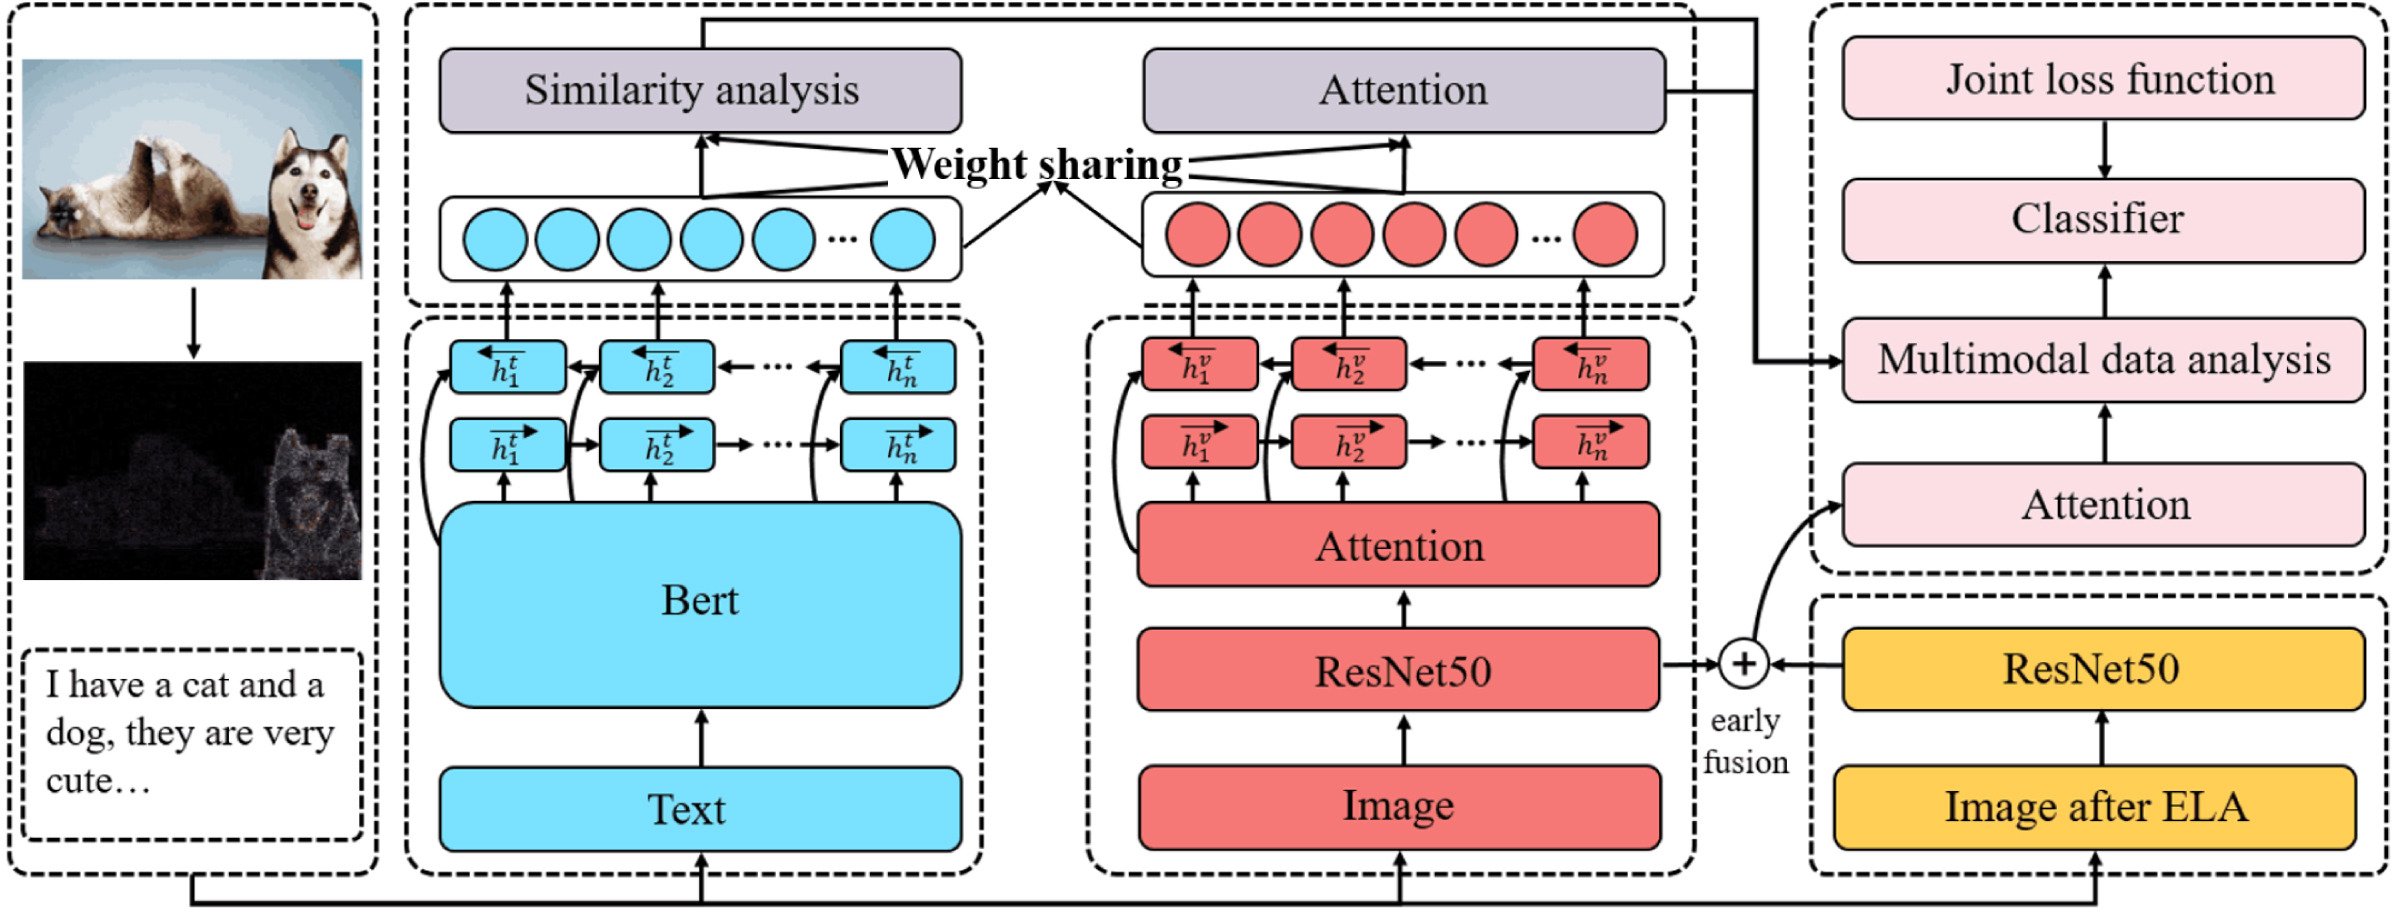
\includegraphics[width=0.8\linewidth]{MCNN-model-architecture.jpg}
    \caption{Note. Figure depicts the architecture of the proposed MCNN model. The module coloured blue is the text feature extraction model; the module coloured red is the visual semantic feature extraction module; the module coloured in purple (above the text and visual semantic feature extraction modules) is the similarity measurement module; the module in yellow/orange is the visual tampering feature extraction module; and lastly the module in pink is the multimodal fusion module. From "Detecting fake news by exploring the consistency of multimodal data", by \citeauthor{mcnn}, 2021, \textit{Information Processing and Management.}, 58(5), https://doi.org/10.1016/j.ipm.2021.102610. Copyright 2024 held by 2021 Elsevier Ltd.}
    \label{fig:placeholder}
\end{figure}

%check figure citation before submission, i think i fucked up on the page numbering here (i replaced with doi but unsure where the doi goes)

\parencite{graph-attention-multimodal} proposed a new model for detecting fake news, the "Domain-Adversarial \& Graph Attention Neural Network" or DAGA-NN. This approach is multimodal and takes both image and text as input. The proposed model was designed in order to address the challenge machine learning approaches faced when attempting to classify cross-domain news samples that did not (or had few instances of) appear in its training data. The architecture is depicted in figure 4. Starting with the feature extractor module, the text component is first cleaned and tokenised before being passed to a BERT model to gain vector representations which are then passed to the Bi-LSTM to capture information about the text and temporal features. As for the image feature extraction, the input image is fed to a pre-trained VGG19 model and the output is passed to a fully connected neural network to gain the feature representation of the image. The text and image features are then fused together to form a single representation of the image and text. The fused feature representation is then fed to the domain discriminator whose goal it is to determine the domain information of the input news. The model is designed in such a way that the domain discriminator is put in competition with the feature-extractor module, forcing the module to output features which are not (or at least minimally) domain-specific, which helps the classifier train on features not dependent on domain and increasing its cross-domain classification accuracy. The domain discriminator is a two-layer neural network which outputs a vector of k-dimensions representing its probability of belonging to each of the k domains. Moving on to the graph-attention-based-classifier, it first takes news articles and creates a graph of them. Edges are drawn between nodes if their cosine similarity is high. Once the graph is built, the graph attention layer learns the importance of each node's neighbours when classifying an input article. This is critical as during this phase, the graph attention layer will strengthen connections between nodes (articles) which are similar semantically and have the same veracity label (true or false) and vice versa (weaken connections if veracity label is opposing). This establishes clear boundaries between real and fake news, even if they are semantically similar. The DAGA-NN model was tested against two datasets, the Twitter and Weibo datasets and managed to outperform state-of-the-art models. The DAGA-NN model was able to achieve macro F1-scores of 0.8828 and 0.9522 for the Twiier and Weibo datasets respectively. The best baseline model the DAGA-NN model was tested against was the Event Adversarial Neural Network or EANN and it outperformed it by 0.0890 - 0.0112 in terms of macro F1-score. 

\begin{figure}[H]
    \centering
    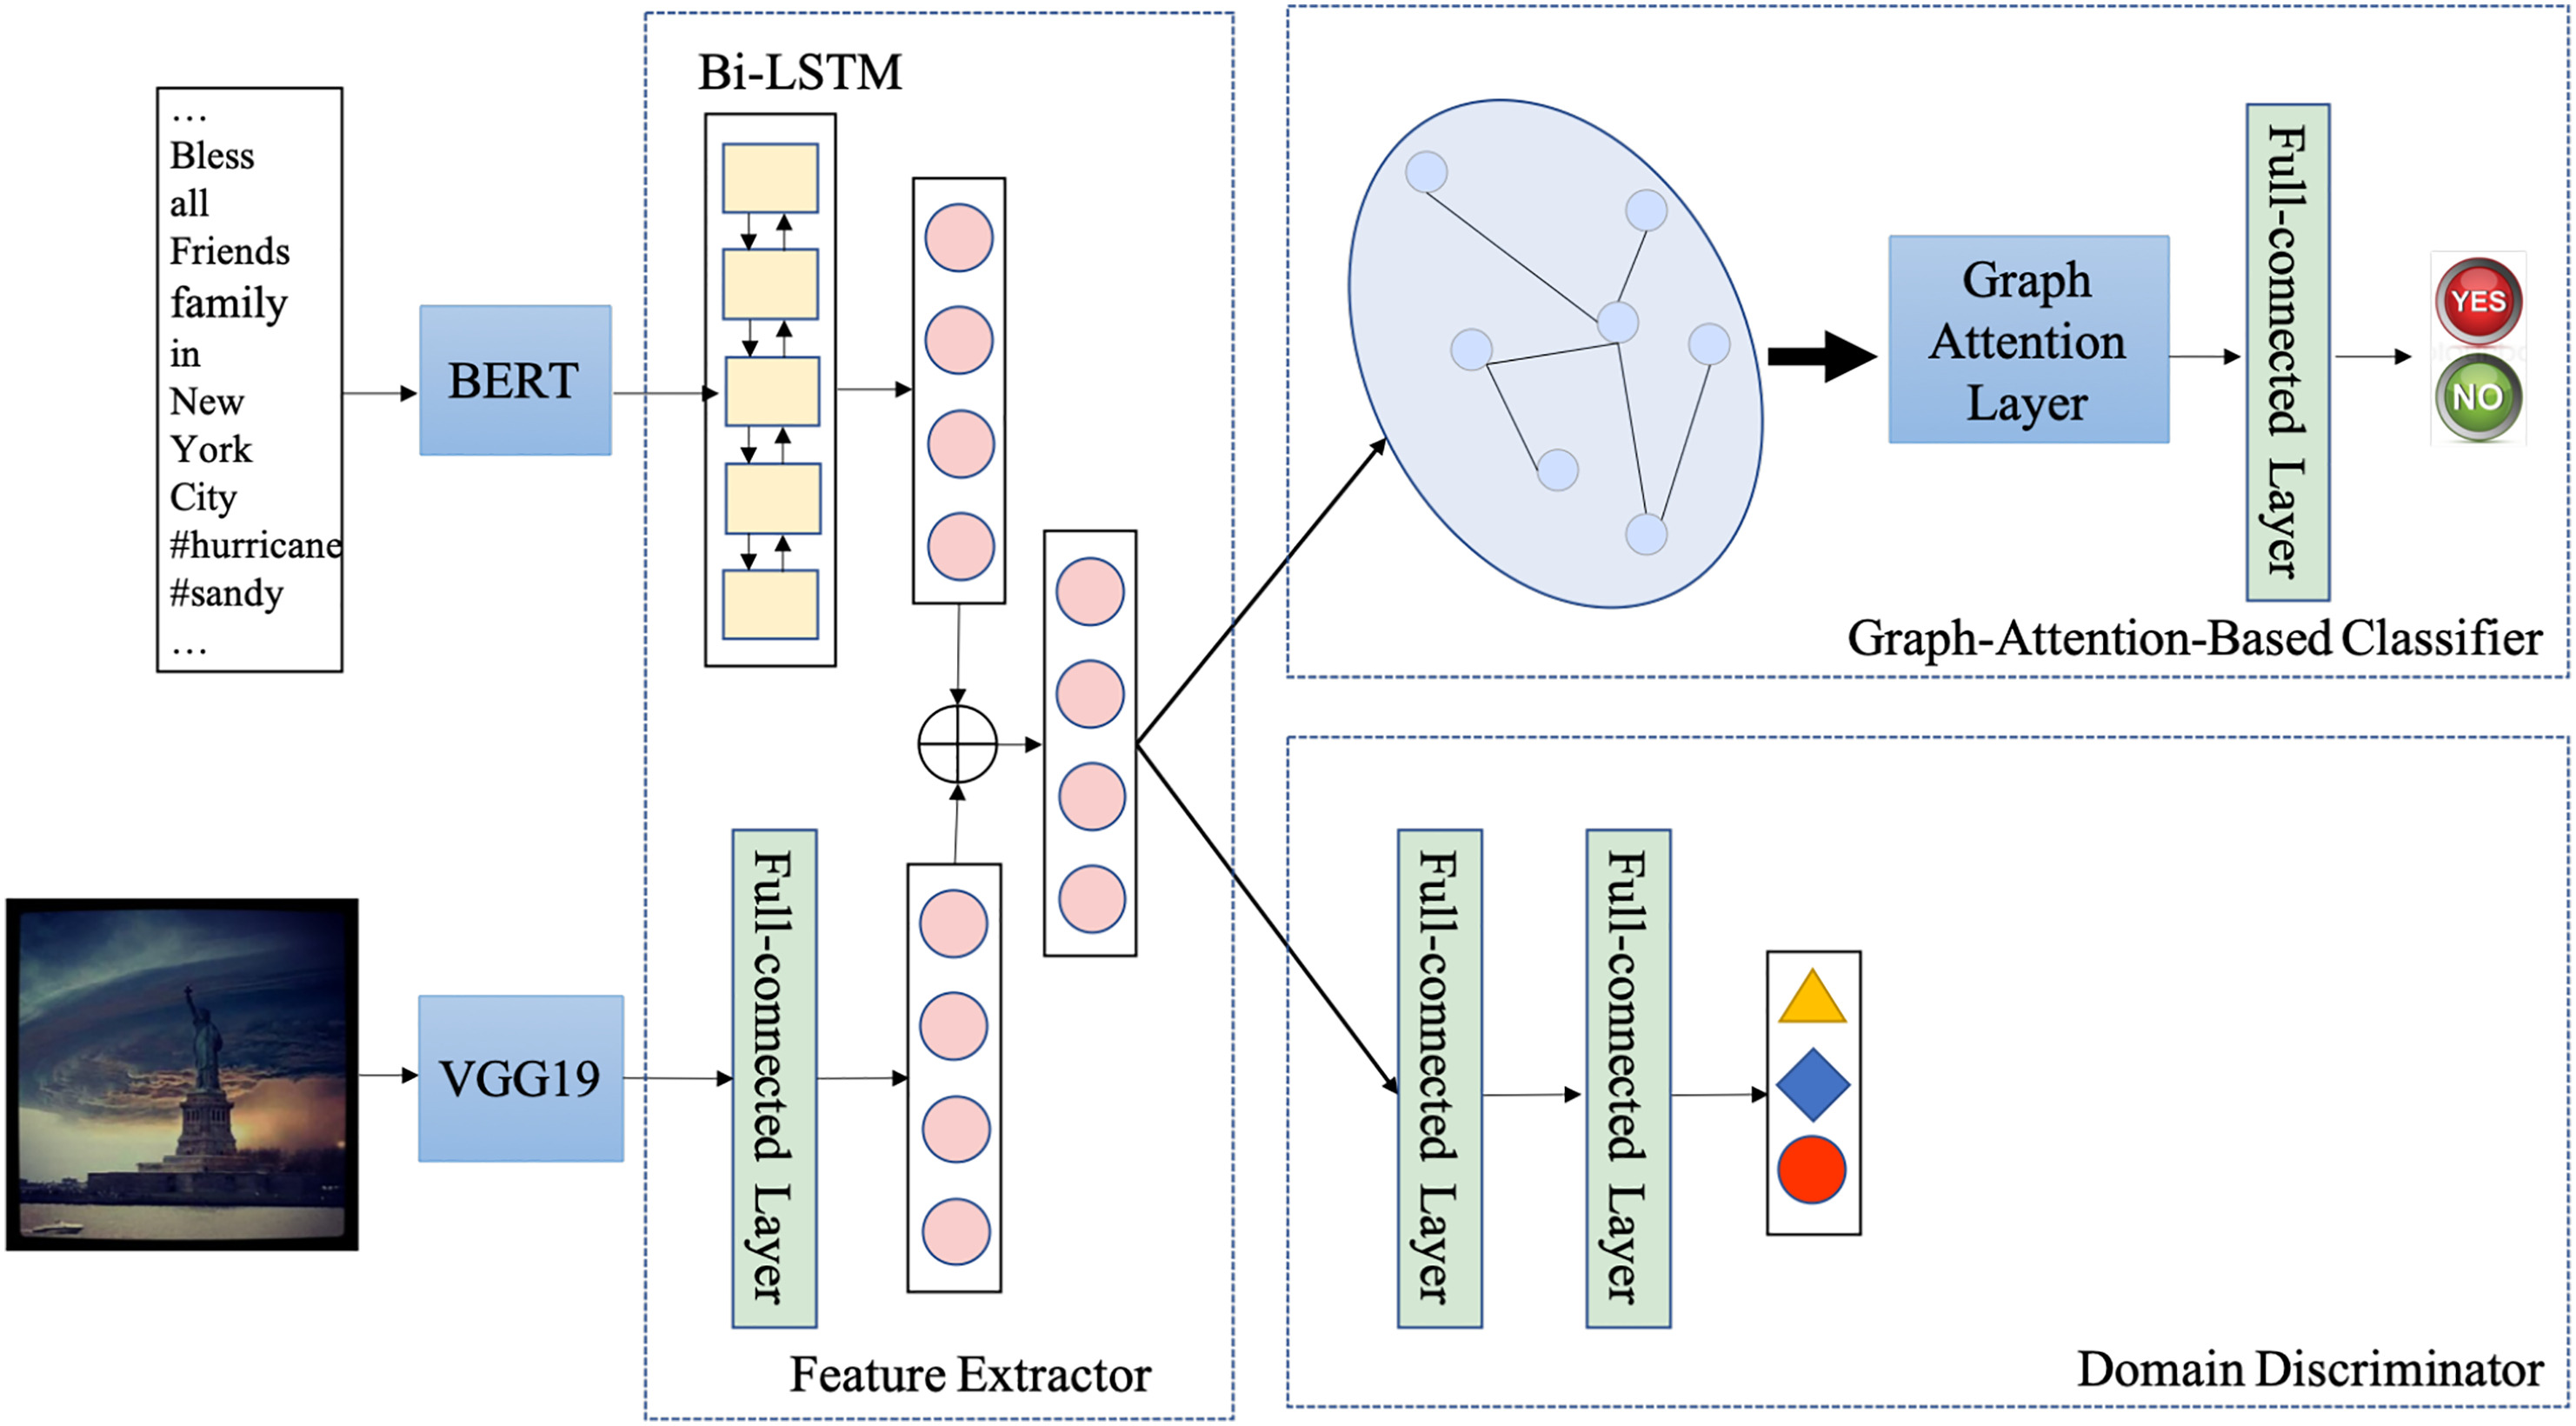
\includegraphics[width=0.5\linewidth]{graph-based-architecture.jpg}
    \caption{Note. Figure depicts the architecture of the DAGA-NN model, each box represents a module which is labelled in the buttom right corner. From "Improving fake news detection with domain-adversarial and graph-attention neural network" by \citeauthor{graph-attention-multimodal}, 2021, \textit{Decision Support Systems}, 151, p. 3 (https://doi.org/10.1016/j.dss.2021.113633). Copyright 2021 Elsevier B.V.}
    \label{fig:DAGA-NN Architecture}
\end{figure}

%Note. Explanations to supplement or clarify information in the image. From [or Adapted from] “Title of Article,” by First Initial. Second Initial. Author Surname, Year, Journal Title, Volume(Issue), page number (url or doi if from an ejournal). Copyright Year by Name of Copyright Holder [or In the public domain or Creative Commons license abbreviation]. Reprinted with permission. [or Adapted with permission.] if permission is sought and obtained.



\subsubsection{Language Model Approaches}
The rise of Large Language Models (LLMs) have complicated detection of fake news, to this end \parencite{sheepdog} proposed a new model "SheepDog" leveraging LLMs to improve detection. The model utilises two different models, an LLM for news re-framing and a fine-tuned language model for classification. Firstly, SheepDog utilises an LLM to transform news content into different styles so as to remove stylistic with varying prompts in order to transform a dataset into one which there is minimal stylistic differences between real and fake news. Then the LLM is further prompted with a set of questions to which the LLMs responses are used as pseudo-labels. Moving on to the language model stage, the language model is fine-tuned using labelled datasets processed by the LLMs. The language model will take input from the LLM stage and output the prediction (true or false news). SheepDog is designed to be able to work with any language model and as such the authors tested the SheepDog framework with several language models. For evaluation the authors tested SheepDog against LLM-empowered style attacks, unperturbed (original) articles, and adaptability with different language models. For the baseline models SheepDog was compared againts, the authors used three main groups of models: text-based fake news detectors, fine-tuned language models and LLMs. And the researchers used three datasets: PolitiFact, GossipCop and LUN. Sheepdog proved to be resilient against LLM-empowered style attacks and its performance was superior to all baseline models. When tested against unperturbed articles, SheepDog had comparable or superior performance relative to the baseline models with F1-scores of between 0.9304 - 0.7575. As for adaptability with various language models, the SheepDog framework was able to improve the performance of these language models. The best language model which was used as a backbone in the SheepDog framework depended on which dataset they were tested against but all language models integrated into the SheepDog framework performed better than its unintegrated counterpart with F1-scores of between 0.7354 - 0.8563 compared to the (unintegrated; lone) language models which had F1-scores between 0.5247 - 0.7617. \\

\subsubsection{Explainable Models}
Research by \textcite{xai-bert} proposed a novel approach which sought to make the model's decision making explainable (explainable AI), the reason being that having a black-box system determine the veracity of something doesn't inspire confidence, something an explainable AI model could mitigate. The researchers utilised DistilBERT which is a lighter variant of BERT, combined with an LSTM layer, a pooling layer, dense feed forward layer and finally the output layer. They then attached an explainability module to the black-box classifier. This module is composed of two post-hoc explainable AI techniques, Local Interpretable Model-Agnostic Explanations (LIME) and Anchors. Post-hoc refers to techniques which attempt to give some level of transparency to an otherwise black-box model. LIME works by sampling the model in the vicinity of a prediction (imagine having an unknown 'X' on a spot on a graph and then picking spots around it to approximate the 'X''s coordinates) and the response to the sampling is used to train a linear model that approximates the model's prediction that can be interpreted. While Anchors refer to an algorithm that applies 'rules' to local predictions, the rules being 'if-then' statements which should ensure that any prediction will remain the same wherever the rule holds. The model was able to achieve 0.98 F1-score for both positive and negative classes. The researchers were able to conclude from the results that it is feasible to use methods such as LIME and Anchors to explain the models behaviour. Although there was some overlap between LIME and the Anchors when explaining the model's behaviour, the results showed it is possible to use multiple types of these methods can be used to derive explanations. \\

\textcite{Xflag} proposed an explainable AI approach, XFlag, to fake news detection which sought to increase the transparency and trust of black-box AI models. The authors used the Weibo dataset, which was processed to extract content, user and sentiment features. Content features were extracted with Doc2Vec which generates word embeddings from the content, similar to BERT, albeit Doc2Vec is an older model. User features were extracted from the user's profile, such as followers, location, etc.. Sentiment features were extracted with the Google Cloud Natural Language API which returned the emotional, "sentimental" data from the content. These features are then passed to fully connected layers before being passed to the LSTM in order to standardise the input to the LSTM. XFlag was able to perform comparably to state of the art models, with an F1-score of 0.938. As for the explainability, the authors used the Layer-wise Relevance Propogation (LRP) algorithm which uses reverse propagation, essentially start with the model output and going in the reverse direction through the model's various layers to determine which neurons had the most impact on the result. The output of the LRP would be the model's (being tested) input shape but with the relevance score for each neuron, this is known as the explanation vector. LRP was applied to the XFlag model after the model was trained, and the output explanation vectors are then passed to Situation Awareness-based Agent Transparency (SAT) framework, specifically the SAT-3 (the researchers used other SAT versions from SAT 1 - 3 which each iteration having more insightful explanations, SAT-3 was most preferred by users) which takes this raw data and processes it in order to generate visualisations, textual annotations and the model's uncertainty so that the user can see how the model came to the conclusion that it did. Users were tested on their trust of the XFlag model with various SAT versions, the lowest being SAT-1 which, similar to a model with no explainability, output the result without deeper explanation. The results were that users reported highest satisfaction and trust as the SAT level and correspondingly, the depth of the explanations of the model's prediction, increased, the highest being SAT-3. \\


Research by \textcite{xai-bilstm} explored the use of explainable AI (XAI) for detection of toxic COVID-19 fake news, proposing the Toxic Fake News Detection System (TFNDS) which uses Bidirectional Long Short Term Memory (BiLSTM) for classification and similar to \textcite{Xflag} the authors used LIME to explain the black-box model (the BiLSTM). The authors used two datasets which they subsequently merged together, the data was then preprocessed with removal of stop words, removal of emojis, removal of repetitive posts, lemmenisation and etc.. This data is then passed to a scikit-learn (also known as sklearn) pipeline where lists of words are indexed and turned into lists of indices and the length of this list is standardised by a transformer to a maximum length of 100. This is then passed to the model which is composed of 128 BiLSTM hidden units followed by 3 dense layers with a Sigmoid output layer for the final classification. As for the explainable section, LIME augments the data by removing features to see which features (words) was most important to the output and this information is visualised by highlighting the words. On the primary dataset used, the model was able to achieve an F1-score of 0.9425 and when tested on an additional dataset for verification (WNUT-2020) it achieved an F1-score of 0.894 which outperformed all other machine learning and deep learning models the authors built. The authors also sought to ensure the LIME explanations were correct, this was done by constructing a pipeline to find the Pointwise Mutual Information (PMI) of words throughout the entire dataset (in contrast to LIME which is local) and their association with a real or fake class. To conduct the evaluation, the 20 most important words for each post as found by LIME and extracted and compared to their rank in the PMI ranking using Kendall's Tau correlation coefficient. The Kendall's correlation for the BiLSTM was 0.35, the authors noted that the general range for Kendall's Tau coefficient was between 0.3 and 0.4, indicating that the LIME explanations had issues with allignment as the PMI context is global while LIME is local. \\


\subsubsection{Fine-tuning Approaches}

An issue with current models is that while they work well with data which was found in their training sets, they often suffer in performance when they encounter data unknown to them \parencite{BERT-finetuning}. To solve this issue, \textcite{BERT-finetuning} proposed a novel approach, Feature Regularization-based Adversarial Fine-tuning (FGM-FRAT). This approach generates perturbed versions of the input in order to confuse the model. This forces the model to find new, deeper patterns instead of relying on otherwise superficial features. The key innovation however, is the addition of a regularization term to the loss function which seeks to minimise the difference between the features generated from the unperturbed, original text with the features generated from the perturbed text. This ensures the feature representation generated by the model will remain similar between original and perturbed text, improving generalisation. The authors used the FakeNewsNet dataset to fine-tune a BERT model using the FGM-FRAT approach using the FakeNewsNet dataset. The authors then tested the fine-tuned model with unseen datasets (BuzzFeedNews, LIAR, WELFake and KaggleFakeNews), using the standard BERT model as a baseline as well as some other fine-tuned BERT models which were fine-tuned with various approaches. The BERT-FGM-FRAT model performed the best amongst all models tested, with improvements of up to 0.32 in terms of F1-score against the base BERT model on the BuzzFeedNews dataset. While for other datasets the BERT-FGM-FRAT managed to offer sigificant performance improvements with the sole exception of the WELFake dataset where it was only able to improve upon the base model incrementally with a 0.03 (F1-score) improvement. \\

\subsubsection{Graph-based Approaches}
Methods which seek to analyse propagation structure for fake news detection often use graph-based methods which overlook the semantic information being propagated, while methods which analyse the semantic information of the content usually fail to understand the propagation structure \parencite{GBCA}. Research by \textcite{GBCA} proposed a novel approach, Graph Convolution Network and BERT combined with Co-Attention (GBCA) which seeks to combine graph based analysis of propagation techniques while using BERT for semantic analysis in order to classify fake news. To capture the spread of news, the proposed model constructs two graphs to capture propagation and dispersation using Edged-enhanced Bayesian Graph Convolution Network (EBGCN). For semantic feature extraction, the GBCA uses a pre-trained BERT to generate vectors from the content which capture the semantic data. And finally to integrate the two approaches, the authors used a co-attention mechanism which computes an affinity matrix to find the relationship between the features from both the structural (propagation and dispersion) and semantic features, the co-attention mechanism will then dynamically assign weights to the features. The authors used three datasets, Twitter15, Twitter16, and PHEME; and used baseline methods including GRU-RNN, SVM-TK (Support Vector Machine - Tree Kernel) among other graph-based methods and deep learning methods. GBCA managed to outperform all models it was compared against in terms of accuracy with a score of 92.8\%, 90.3\% and 70.8\% for the Twitter15, Twitter16, and PHEME datasets respectively; however it was beaten by several Graph Comvolution Networks (GCNs) when it came to F1-score for some of the classes. Despite this, it is worth noting the GBCA was more computationally efficient when training as the co-attention module used reduced the amount of iterations required for convergence. \\


%This processed data was then analysed for toxicity using the Detoxify Python package and this would output a vector of size 9, containing 7 toxicity attributes (sexually explicit, obscene, insult and etc.) as well as the toxicity and non-toxicity score. Depending on the toxicty score, the dataset is then labelled toxic or non-toxic. 

\subsection{Summary}
\begin{landscape}
\begin{table}[H]
\tiny
\centering
\caption{Summary of Literature Review Findings}
\label{tab:lit_review_summary}
\begingroup
\setlength{\tabcolsep}{4pt} % Adjust horizontal space between columns
\renewcommand{\arraystretch}{1.2} % Adjust vertical space between rows

% Define the table environment.
% The total width is \textwidth.
% The column specifiers (l, X, p{...}) are defined below:
% l: Left-aligned (good for Author/Year)
% X: Automatically adjusts width (good for Title, Findings, Notes)
% c: Center-aligned
\begin{tabularx}{\linewidth}{@{} c l X X X X X l @{}}
    \toprule
    \textbf{Author(s)} & \textbf{Year} & \textbf{Title} &  \textbf{Model Proposed} & \textbf{Proposed Methodology} & \textbf{Results} & \textbf{Notes} & \textbf{BERT used?} \\
    \midrule
    % --- Row 1 ---
    \textcite{cnn_chinese} & 2023 & \citetitle{cnn_chinese} &  Convolutional Feed-Forward (Conv-FFD) & Use of CNN to learn relationships and ultimately classify based on sentence-level embeddings generated by a "sliding window" & F1-scores of between 0.8702 - 0.8855. & Researchers one-hot-encoded Chinese characters, a technique not feasible for English text. & No \\
    \addlinespace
    % --- Row 2 ---
    \textcite{opcnn-fake} & 2021 & \citetitle{opcnn-fake} & Optimized Convolutional Neural Network to Detect Fake News (OPCNN-FAKE) & Use of GLoVe to produce word embeddings which are then use to train the OPCNN-FAKE model. & F1-scores of between 0.959 - 0.9999 & Extremely high scores on ISOT dataset indicate some level of overfitting. & No \\
    \addlinespace
    % --- Row 3 ---
    \textcite{hybrid_cnn-lstm} & 2024 & \citetitle{hybrid_cnn-lstm} & CNN-LSTM & Use of FastText to produce word embeddings which is then used to train a CNN-LSTM hybrid. & F1-scores of between 0.91 - 0.99 & - & No \\
    \addlinespace
    % --- Row 4 ---
    \textcite{hybrid2} & 2024 & \citetitle{hybrid2} & Bidirectional Long Short Term Memory – Bidirectional Gated Recurrent Unit (Bi-LSTM – Bi-GRU) & Researchers used FastText to generate embeddings which was used to train the hybrid model. & F1-scores of between 0.98 - 0.99 & Research was done on Arabic text & No \\
    \addlinespace
    % --- Row 5 ---
    \textcite{gbert} & 2024 & \citetitle{gbert} & Generative Bidirectional Encoder Representations from Transformers (GBERT) & Use of BERT to generate word embeddings and GPT to generate global vectors. Outputs from BERT and GPT are subsequently combined and passed to a classifier. & F1-score of 0.9623 & Researchers also experimented with XGBoost which performed nearly on par with GBERT in terms of accuracy. & Yes \\
    \addlinespace
    % --- Row 6 ---
    \textcite{deep-ensemble} & 2022 & \citetitle{deep-ensemble} & Deep Ensemble (Stacking) & Use of SDL models as base models and multilevel-perceptron classifier at the top. & F1-score of 1.00 for ISOT F1-scores of 0.48 - 0.82 for LIAR & LIAR dataset has more than 2 classes & No \\
    \addlinespace
    % --- Row 7 ---
    \textcite{traditional-ml} & 2021 & \citetitle{traditional-ml} & Various Machine Learning Models & ML models fitted onto preprocessed datasets with key features extracted during processing & Accuracy of 0.73 (Best model; XGBoost) & - & No \\
    \addlinespace
    % --- Row 8 ---
    \textcite{multimodal} & 2023 & \citetitle{multimodal} & Multimodal Progressive Fusion
    Approach (MPFN) & BERT for text feature extraction, visual feature extractor component for images and these two components are combined using the progressive multimodal feature fusion process. & F1-scores between 0.889 - 0.740 & Multimodal approach & Yes \\
    \addlinespace
    % --- Row 9 ---
    \textcite{mcnn} & 2021 & \citetitle{mcnn} & Multimodal Consistency Neural Network (MCNN)& A 5-module multimodal model using BERT for the text module, ResNet50 and ELA for the image modules with a final softmax classifier. & F1-scores between 0.968 - 0.831 & Multimodal approach & Yes\\
    \addlinespace
    % --- Row 10 ---
    \textcite{graph-attention-multimodal} & 2021 & \citetitle{graph-attention-multimodal} & Domain-Adversarial \& Graph Attention Neural Network (DAGA-NN) & Multimodal model using BERT and a Bi-LSTM for text and VGG19 with a neural network for images, features are then fused (features generated will not be domain-specific, due to adversarial training against the domain discriminator) and passed to the graph-attention-based-classifier. & F1-scores of 0.8828 and 0.9522 & Multimodal with features trained adverarially to be domain-neutral & Yes \\
    \addlinespace
    % --- Row 11 --- COME BACK TO THIS AHHHHHHHHHH
    \textcite{sheepdog} & 2024 & \citetitle{sheepdog} & SheepDog & SheepDog leverages LLMs to remove stylistic differences in the dataset which is passed to a fine-tuned language model for classification. & 0.7354 - 0.8563 (tested on perturbed dataset) & SheepDog is technically a framework & No \\
    \addlinespace
    % --- Row 12 ---
    \textcite{xai-bert} & 2021 \citetitle{xai-bert} & DistilBERT-LIME (Unnamed by authors) & The proposed model used DistilBERT with several other layers for fake news classification, with Anchors and LIME being used to explain the otherwise black-box algorithms. & F1-score of 0.98 & Used variant of BERT  & Yes \\
    \addlinespace
    % --- Row 13 ---
    \textcite{Xflag} & 2022 & \citetitle{Xflag} & XFlag & XFlag utilised Doc2Vec to extract features from the content, sentiment-features were extracted by a Google API, and user features from their profile. These were used to train an LSTM which was made explainable by the LRP algorithm. & F1-score of 0.938 & Model considered more than just text and considered sentiment and user information as well. & No \\
    \addlinespace
    % --- Row 14 ---
    \textcite{xai-bilstm} & \citeyear{xai-bilstm} & \citetitle{xai-bilstm} & Toxic Fake News
    Detection System (TFNDS) & Used Bi-LSTM in combination with LIME for explainability. Additionally attempted to evaluate accuracy of LIME using PMI. & F1-scores of 0.9425 and 0.894; Kendall's Tau Coefficient of 0.35 & PMI evaluation likely had issues of allignment. & No\\
    \addlinespace
    % --- Row 15 ---
    \textcite{BERT-finetuning} & 2023 & Boosting generalization of fine-tuning BERT for fake news detection & FGM-FRAT & Fine-tuning using an adversarial approach can substantially improve generalisation of models & Improvements in performance of between 0.32 and 0.03 (F1-score) relative to base BERT model & \textbf{-} & No \\
    \addlinespace
    % --- Row 16 ---
    \textcite{GBCA} & \citeyear{GBCA} & \citetitle{GBCA} & Graph Convolution Network and BERT combined with Co-Attention (GBCA) & GBCA builds graphs to capture the dissemination of news and BERT to process the content. These approaches are fused together with a co-attention mechanis. & Accuracy of 92.8\% - 70.8\% & \textbf{-} & Yes \\
    \addlinespace
    \bottomrule
\end{tabularx}
\endgroup
\end{table}
\end{landscape}

\section{Research Methodology}
\subsection{Datasets}
\subsubsection{WELFake Dataset}
The WELFake dataset was downloaded from Kaggle, and contains 72134 rows of data. The class balance was relatively balanced, with the real news class having an excess of 2000 rows as can be referred to in figure 5. As for features, the dataset came with four columns, an unnamed ID column, title (of the news article), text (from the news article) and the label (real/fake). There were 558 missing values in the 'title' column and 39 missing values in the 'text' column intitially.

\begin{figure} [H]
    \centering
    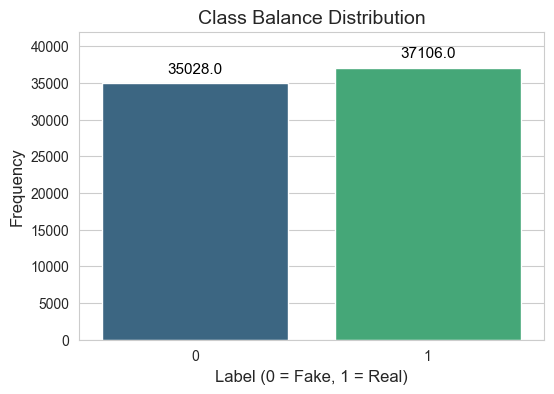
\includegraphics[width=0.5\linewidth]{WELFake class distribution.png}
    \caption{Note. Figure depicts the class distribution of the WELFake dataset}
    \label{fig:placeholder}
\end{figure}

\subsubsection{Fake News Classification}
This dataset, named "Fake News Classification" was downloaded from Kaggle. It contains 40597 rows of data with 4 columns: an unnamed ID column, title, text and label. There were no missing values or duplicates in any of the rows initially before pre-processing. And the class balance had an excess of approximately 3000 in favour of the positive class (real). 

\begin{figure} [H]
    \centering
    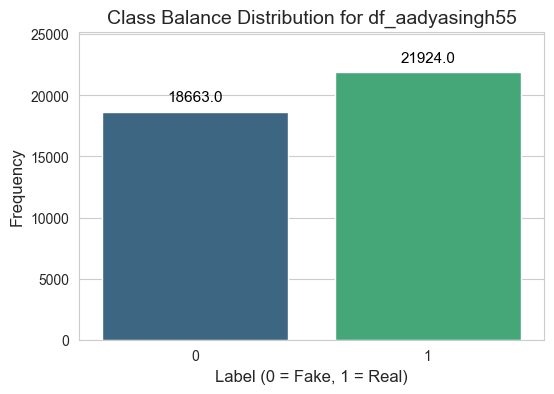
\includegraphics[width=0.5\linewidth]{Fake news classification class balance.png}
    \caption{Note. Figure depicts the class distribution of the Fake News Classification dataset}
    \label{fig:placeholder}
\end{figure}

\subsubsection{FakeNewsNet}
The FakeNewsNet dataset was downloaded from Kaggle, it is worth noting this was not the original dataset, it had been its various csv files merged by the uploading user "algord". FakeNewsNet contains 23196 rows, with 5 columns: title, news\_url, source\_domain, tweet\_num and label. The dataset contained missing values in the news\_url and source\_domain columns (which is acceptable as this is not required later on in training or testing). There were 137 duplicate rows (which will be dropped later on) initially. The class balance was heavily skewed in favour of the positive (real) class, with approximately 75\% of all rows belonging to the positive class. 

\begin{figure} [H]
    \centering
    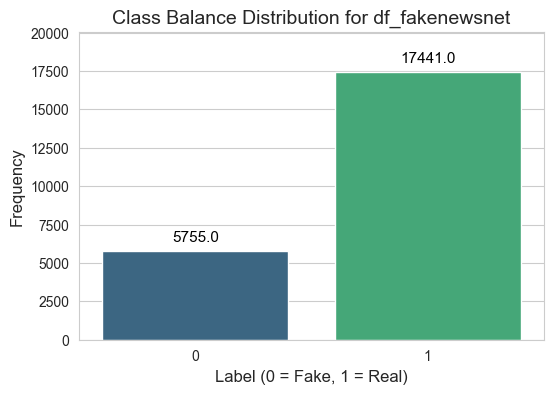
\includegraphics[width=0.5\linewidth]{FakeNewsNet class distribution.png}
    \caption{Note. Figure depicts the class distribution of the FakeNewsNet dataset}
    \label{fig:placeholder}
\end{figure}

\subsubsection{Fake News Detection}
The Fake News Detection dataset was downloaded from Hugging Face. It contains 44267 rows and 6 columns: Unnamed ID column, title, text, subject, date, and label. There were no missing values or duplicate rows initially. The class balance is relatively balanced with the difference between the positive and negative classes being approximately ± 3\%. 

\begin{figure} [H]
    \centering
    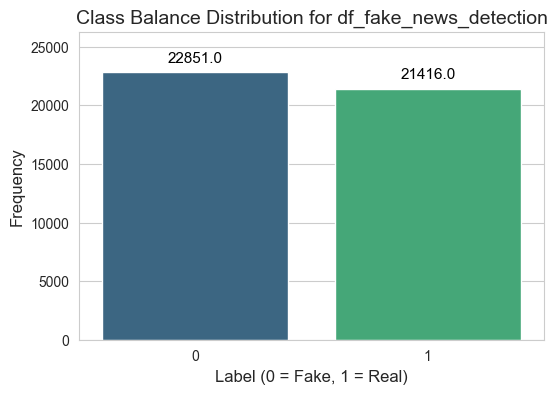
\includegraphics[width=0.5\linewidth]{fake news detection class balance.png}
    \caption{Note. Figure depicts the class distribution of the Fake News Detection dataset}
    \label{fig:placeholder}
\end{figure}

\subsubsection{ISOT}
The ISOT dataset was downloaded from the University of Victoria website. It contains 44898 rows with 5 columns: title, text, subject, date and label. There were no missing values initially. However there were 209 duplicate rows initially. The class balance was relatively balanced, with the difference in proportion of the positive and negative classes being approximately ± 5\%.

\begin{figure} [H]
    \centering
    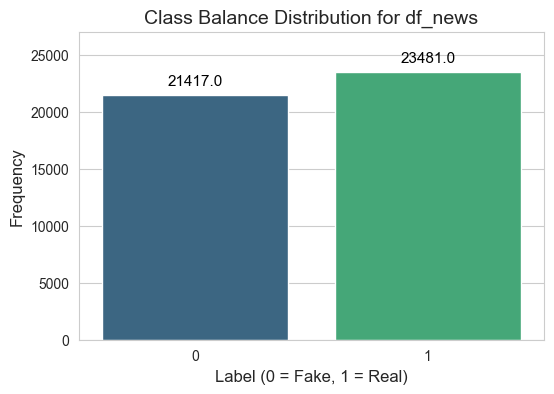
\includegraphics[width=0.5\linewidth]{ISOT class balance.png}
    \caption{Note. Figure depicts the class distribution of the ISOT dataset}
    \label{fig:placeholder}
\end{figure}

\subsection{Data Understanding}

\subsection{Data Pre-processing}
The data was processed by first merging 'title' and 'text' columns together if the dataset had split 'title' and 'text' into different columns, this would be combined. In one of the datasets "FakeNewsNet", only the 'title; column was used. After the columns were combined, the new 'combined\_text' column was checked for missing strings and null values, of which none were found.

After combining the columns, any columns that did not contain the label or 'combined\_text' column were dropped, such as source URLs columns, and other metadata like date. This revealed substantially more duplicated rows, likely as a result of the datasets being gathered through scraping methods which scraped the same content from multiple sources causing the dataset to have duplicated textual columns but different metadata, which allowed it to evade detection earlier. The total number of samples dropped is summarised in table X. %name the table when done

Once completed, the 'combined\_text' column was stripped of any non-unicode characters as well as links, phone numbers and other non-ASCII characters. The removal of non-ASCII characters is possible as this research focuses on English news. After this, any rows with empty strings are removed. 

\begin{table}[H]
    \centering
    \scriptsize % Reduces font size slightly to fit width
    \setlength{\tabcolsep}{3pt} % Reduces space between columns
    \caption{Summary of Data Preprocessing Statistics}
    \label{tab:preprocessing_stats}
    \begin{tabular}{l cc cc cc cc}
        \toprule
         & \multicolumn{2}{c}{\textbf{Initial}} 
         & \multicolumn{2}{c}{\textbf{After Combining Text}} 
         & \multicolumn{2}{c}{\textbf{After Dropping Rows}} 
         & \multicolumn{2}{c}{\textbf{After Cleaning}} \\
        \cmidrule(lr){2-3} \cmidrule(lr){4-5} \cmidrule(lr){6-7} \cmidrule(lr){8-9}
        \textbf{Dataset} & \textbf{Missing*} & \textbf{Duplicates} & \textbf{Missing*} & \textbf{Duplicates} & \textbf{Missing*} & \textbf{Duplicates} & \textbf{Missing*} & \textbf{Duplicates} \\
        \midrule
        WELFake & 597 & 0 & 0 & - & - & 8458 & 6 & - \\
        Fake News Classification & 0 & 0 & 0 & - & - & 2 & 5 & - \\
        FakeNewsNet & 660 & 137 & 0 & - & - & 1349 & 3 & - \\
        Fake News Detection & 0 & 0 & 0 & - & - & 5612 & 5 & - \\
        ISOT & 0 & 0 & 0 & - & - & 5795 & 5 & - \\
        \bottomrule
    \end{tabular}
    \par\medskip
    \raggedright
    \footnotesize{\textit{Note.} (-) indicates metric not checked at this stage. \\
    (\*) Shows the sum of missing values, not necessarily the number of rows (in stages after Initial, only \texttt{combined\_text} is checked).}
\end{table}

\begin{table}[H]
    \centering
    \caption{Dataset Shapes (Initial vs. Final)}
    \label{tab:dataset_shapes}
    \begin{tabular}{l c c}
        \toprule
        \textbf{Dataset} & \textbf{Initial Shape} & \textbf{Final Shape} \\
        \midrule
        WELFake & (72134, 4) & (63670, 2) \\
        Fake News Classification & (40587, 4) & (40580, 2) \\
        FakeNewsNet & (23196, 5) & (21844, 2) \\
        Fake News Detection & (44267, 6) & (38650, 2) \\
        ISOT & (44898, 5) & (39098, 2) \\
        \bottomrule
    \end{tabular}
\end{table}


\begin{figure} [H]
    \centering
    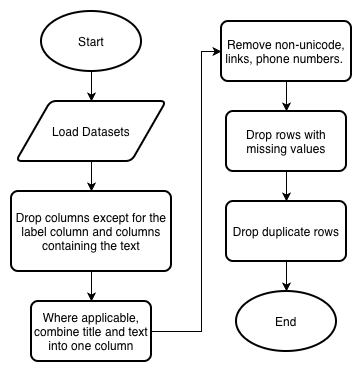
\includegraphics[width=0.5\linewidth]{FYP_Research_Methodology.png}
    \caption{Note. Figure depicts preprocessing steps in flowchart form}
    \label{fig:preprcessing_flowchart}
\end{figure}


After the above processes, the data was then processed seperately depending on the type of model being trained. For BERT, the data was tokenised using BERT's tokeniser without further processing steps. For GLoVe, the data was decapitalised and then split into individual words for processing. Whereas for Word2Vec, the data was both decapitalised and lemmenised before the data is used to train the Word2Vec model. 

\begin{table}[H]
\centering
\caption{Summary of Additional Preprocessing Steps for Each Model Type}
\label{tab:preprocessing}
\begin{tabular}{@{}lp{10cm}@{}}
\toprule
\textbf{Model Type} & \textbf{Preprocessing Steps} \\
\midrule
BERT & Tokenization using BERT's tokenizer (no additional preprocessing) \\
\addlinespace
GLoVe & \begin{itemize}[leftmargin=*, nosep]
    \item Decapitalization (lowercase conversion)
    \item Splitting into individual words
\end{itemize} \\
\addlinespace
Word2Vec & \begin{itemize}[leftmargin=*, nosep]
    \item Decapitalization (lowercase conversion)
    \item Lemmatization
    \item Splitting into individual words
\end{itemize} \\
\bottomrule
\end{tabular}
\end{table}

\subsection{Modelling}
Modelling depended on which kind of embedding was used. For BERT, fine-tuning was used to fine-tune a base BERT-uncased model into a 2-label classification model. For GLoVe and Word2Vec, after the datasets were turned into embeddings, the now vectorised datasets were fitted to machine learning models and used to train several deep-learning models as well, specifically: CNN, LSTM and CNN-LSTM. 

\begin{table}[H]
\centering
\caption{Summary of Modelling Approaches for Each Embedding Type}
\label{tab:modelling}
\begin{tabular}{@{}lp{10cm}@{}}
\toprule
\textbf{Embedding Type} & \textbf{Modelling Approach} \\
\midrule
BERT & \begin{itemize}[leftmargin=*, nosep]
    \item Fine-tuning to convert BERT into a classification model 
\end{itemize} \\
\addlinespace
GLoVe & \begin{itemize}[leftmargin=*, nosep]
    \item Machine learning models (trained on vectorised datasets)
    \item Deep learning models: CNN, LSTM, CNN-LSTM
\end{itemize} \\
\addlinespace
Word2Vec & \begin{itemize}[leftmargin=*, nosep]
    \item Machine learning models (trained on vectorised datasets)
    \item Deep learning models: CNN, LSTM, CNN-LSTM
\end{itemize} \\
\bottomrule
\end{tabular}
\end{table}

\subsection{Evaluation}
%check tense
Evaluation of the models will be done by comparing F1-score, and its constituent metrics of recall and precision, as well as accuracy. These metrics willbe obtained from the trained models by using the test sets.\\ 

F1-score is a formula which combines precision and recall. Precision describes the proportion of a model's positive predictions and is calculated by dividing the number of \textit{True Positives} by the sum of \textit{True Positives} and \textit{False Positives}. Recall describes the model's ability to identify positive instances and is calculated by dividing the number of \textit{True Positives} by the sum of \textit{True Positives} and \textit{False Negatives}. Together these metrics are combined to form F1-score, which is calculated by dividing \textit{2} by the sum of the inverse of \textit{Precision} and \textit{Recall}. \\

Meanwhile, accuracy is found by dividing the number of correct predictions over the total number of predictions.\\

The formulae described above are also written below in mathematical notation: 

\begin{equation}
\text{Precision} = \frac{\text{True\ Positives}}{\text{True\ Positives} + \text{False\ Positives}}
\end{equation}

\begin{equation}
\text{Recall} = \frac{\text{True\ Positives}}{\text{True\ Positives} + \text{False\ Negatives}}
\end{equation}

\begin{equation}
\text{F1} = \frac{2}{\frac{1}{\text{Precision}} + \frac{1}{\text{Recall}}}
\end{equation}

\begin{equation}
\text{F1} = 2 \times \frac{\text{Precision} \times \text{Recall}}{\text{Precision} + \text{Recall}}
\end{equation}

\begin{equation}
\text{Accuracy} = \frac{\text{Correct\ Predictions}}{\text{Total\ Predictions}}
\end{equation}

\section{Theoretical Framework}


\subsection{Deep Learning Approaches}

\subsubsection{Convolutional Neural Networks}
Convolutional Neural Networks or CNNs are neural networks which generaly have 3 layers: A convolutional layer, pooling layer and a fully-connected layer. The convolutional layer is the key part of a CNN, and it uses a grid of numbers called kernels (or filters) to 'scan' through the various features and perform a mathematical operation known as 'convolution'. After the convolution layer, the pooling layer reduces the size of the data which also helps with reducing the computational demands and also helps with ensuring the model doesn't become focussed on small and irrelevant details. The final, fully-connected layer works by flattening the prior layer's multi-dimensional features into a single layer. This single-layer output can now be fed to a standard neural network for classification.

\subsubsection{Long Short Term Memory}
Long Short Term Memory of LSTMs is a type of Recurrent Neural Network (RNN) which aims to solve an issue with RNNs called the 'Vanishing Gradient Problem'. Essentially, the issue is that RNNs work using gradients which inform the weights in neurons, and these gradients are calculated using the chain rule, which means after dozens of multiplications a gradient will rapidly lose its value. This means that RNNs have 'short term memory', an issue LSTM's solve by selectively holding on to important information in a 'Cell State' through a system of gates. There are three gates: forget gate, input gate, and output gate. The forget gate figures out what information should be forgotten because it is now longer useful. The input gate decides what is worth adding to the 'Cell State'. And lastly the output gate figures out what information in the 'Cell State' is important or relevant to the current situation and outputs that. This ensures that LSTMs are able to hold on to important information over a long-term and doesn't suffer from short-term foregetfulness. This makes LSTMs especially suitable for sequential input where important discriminating features are far between each other. 

\subsection{Embedding Approaches}
\subsubsection{Global Vectors for Word Representation}
Global Vectors for Word Representation or GLoVe is an unsupervised embedding algorithm which generates word embeddings. GLoVe embeddings are pre-trained on massive textual datasets with a pre-set number of dimensions. The training process works by constructing a co-occurence matrix where the rows and columns represent each unique word and each entry in the matrix indicates the frequency of two words occuring next to one another within a predefined context window. So for example, the co-occurence matrix would capture how frequently the words "statistics" and "math" appear together. 

But how is the co-occurence matrix turned into vectors? This takes place during training, each word is assigned a random vector, and then finds the dot product of two vectors (in this case, each vector is a word), then compares it to the logarithm of the co-occurence matrix count (of the two words) to find the error, then depending on the error, the vectors will be updated so it is closer to the logarithm of the co-occurence matrix count. So for example, if two words, "apple" and "fruit" have a logarithm-count of 0.5, and the dot product of their random vector representations returned a value of 0.3, the error would be 0.2 and the model will modify the vectors such that in the next iteration, the dot product will closer align with the logarithm-count. 

But that is not all, if GLoVe only relied on counts in the co-occurence matrix it would encounter issues where common words like "the" become associated with everything and the vectors generated would be less meaningful. To solve this, GLoVe employs weights to ensure the vectors being trained are meaningful. Rare words will be given lower weights (noise), and while common words will have higher weights, there will be a cap so that "the" doesn't unfairly bias the vectors being produced. 

After training these embeddings can be loaded (which is what was done here) and then used to generate embeddings of input text. 

To conclude, GLoVe is an unsupervised algorithm which generates word embeddings based on a massive textual datasets. The vectors produced are representative of the frequency of words relative to other words. 

\subsubsection{Word2Vec}
Word2Vec (Word to Vector) is a neural network embedding model which converts words into dense vector representations. There are two main architectural variants, Continuous Bag of Words and Skip-gram; Skip-gram was used in this instance and thus will be the only variant elaborated on. 

The Word2Vec Skip-gram variant works by trying to predict the words around a single target word. So, using the example of the sentence "I love vanilla ice cream", the target word being the word "vanilla" and the windows being set at two words; the model would focus on trying to predict the words "I", "love", "ice", "cream" around the word "vanilla". 

To do this, the input word (represented in on-hot-encoded form) is taken in by the model as input and passed to the hidden layer and the outputs from this layer is passed to the output layer which tries to guess the words surrounding the input. If the model gets it right, say by correctly guessing the words "ice" and "cream", the connections between these words and the target word is strengthened and if it fails the model will update the weights in the hidden layer so that it will be more likely to guess the correct words in the next iteration.

This massive guessing operation is used to train the hidden layer, so that when the training is complete, the output layer is stripped and the output of the hidden layer becomes the vectors. So to conclude, Word2Vec's Skip-gram variant works by trying to guess words around a target word and through this exercise trains a hidden layer which will be used to turn words into vectors. 

\subsubsection{Bidirectional Encoder Representations from Transformers}
Bidirectional Encoder Representations from Transformers or BERT is a self-supervised bidirectional model which differs from Word2Vec and GLoVe in that while Word2Vec and GLoVe have a single vector for each word; BERT outputs different vectors for each word depending on the context. 

To do this, BERT is trained through two objectives: Masked Language Modelling (MLM) and Next Sentence Prediction (NSP) \parencite{roberta}. MLM works by trying to get BERT to predict the missing word. So using the previous example of "I love vanilla ice cream", say the word "ice" is 'masked' (omitted), BERT will have to try and guess the missing word from: "I love vanilla [mask] cream". Since BERT is bidirectional, it will consider words preceding and subsequent to the mask. This technique gets BERT to learn the relationship between words in a sentence. 

The next technique, NSP is exactly as it sounds. It tries to get BERT to guess if a sentence comes directly after another sentence \parencite{roberta}. So, let's say BERT is given two sentences: the previous example of "I love vanilla ice cream.", and "It tastes so sweet". BERT will have to guess if the latter sentence comes after the former. This was intended to get BERT to learn relationships between pairs of sentences.

However it is important to note that the importance of NSP to BERT may be overstated, as \textcite{roberta} hypothesised after experiments with the NSP component of the loss function showed that removing the NSP loss function could match or even slightly improve performance on downstream tasks. 

In conclusion, the bidrectional nature of BERT gives it an edge and the objectives used to train it, specifically MLM gave it an advantage when understanding context, allowing it to create more meaningful vectors. As a note, BERT does have many variants, including RoBERTa, developed by \textcite{roberta} who were cited earlier; this research uses the original BERT, developed by Google. 

\subsection{Explainable AI Approaches}
\subsubsection{LIME}


\subsection{Classification Models}

\section{Implementation Plan}

\subsection{Experiments}

\subsubsection{GLoVe Embedding}
Experiments involing GLoVe saw the text in the datasets turned into GLoVe embeddings. But first the text in each dataset were turned into lowercase, before being turned into embeddings using weights found in the file 'dolma\_300\_2024\_1.2M.100\_combined.txt'. Each respective dataset and its now converted text was then used to train several machine learning models (KNN, Gaussian NB, Logistic Regression, SVC, XGBoost, Random Forest) and deep learning models (CNN, CNN-LSTM, LSTM). 

Below are tables containing the training parameters for the models trained (both machine learning and deep learning models): 

\begin{table}[H]
    \centering
    \caption{Machine Learning Model Training Hyperparameters}
    \label{tab:ml_model_params}
    \begin{tabular}{l l}
        \hline
        \textbf{Model} & \textbf{Training Arguments} \\
        \hline
        K-Nearest Neighbors (KNN) & \texttt{n\_neighbors=5} \\
        Gaussian Naive Bayes & Default parameters \\
        Logistic Regression & \texttt{max\_iter=1000} \\
        Support Vector Classifier (SVC) & Default parameters \\
        XGBoost & \texttt{use\_label\_encoder=False}, \texttt{eval\_metric='logloss'} \\
        Random Forest Classifier & \texttt{n\_estimators=100}, \texttt{random\_state=42} \\
        \hline
    \end{tabular}
\end{table}

\begin{table}[ht]
    \centering
    \caption{Deep Learning Model Hyperparameters}
    \label{tab:dl_model_params}
    \begin{tabular}{l l l}
        \hline
        \textbf{Model} & \textbf{Parameter} & \textbf{Value} \\
        \hline
        \multicolumn{3}{c}{\textbf{Common Training settings}} \\
        & Epochs & 10 \\
        & Batch Size & 32 \\
        & Learning Rate & 0.001 \\
        & Optimizer & Adam \\
        & Loss Function & BCELoss \\
        & Validation Split & 0.2 \\
        \hline
        \multirow{4}{*}{CNN} & Number of Filters & 100 \\
        & Filter Sizes & [3, 4, 5] \\
        & Dropout & 0.5 \\
        & Activation & ReLU (Hidden), Sigmoid (Output) \\
        \hline
        \multirow{4}{*}{LSTM} & Hidden Dimension & 128 \\
        & Number of Layers & 2 \\
        & Dropout & 0.5 \\
        & Activation & ReLU (Hidden), Sigmoid (Output) \\
        \hline
        \multirow{6}{*}{CNN-LSTM} & CNN Filters & 64 \\
        & CNN Filter Sizes & [3, 4, 5] \\
        & LSTM Hidden Dims & 128 \\
        & LSTM Layers & 1 \\
        & Dropout & 0.5 \\
        & Activation & ReLU (Hidden), Sigmoid (Output) \\
        \hline
    \end{tabular}
\end{table}

\subsubsection{Word2Vec}
Word2Vec experimentation saw the text (from previous processing steps) undergo some final processing which involved turning the text into all lowercase and the text undergoing lemmenisation using the Python library 
NLTK's \textit{WordNetLemmatizer}. After this, the proccessed text was used to train the Word2Vec model for each dataset (as there are 5 datasets, there will be 5 different Word2Vec embedding models).

The training arguments for the Word2Vec models can be found below (note the exact code can not be found in the notebook used for Word2Vec training, but these are the exact arguments used and this snippet was made for simplified viewing of the arguments): 
\begin{lstlisting}[language=Python, caption={Word2Vec Models' Traning Configuration}]
model = Word2Vec(
        sentences=tokenized_texts,
        vector_size=100,
        window=5,
        min_count=2,
        workers=4,
        epochs=10,
        sg=1  # 1 for skip-gram, 0 for CBOW
    )
\end{lstlisting}

After the each Word2Vec model is trained, the models are employed to convert each dataset into embedding-form which can be understood by machine learning and deep learning models. After this process, each respective dataset and its embeddings were then used to train several machine learning models (KNN, Gaussian NB, Logistic Regression, SVC, XGBoost, Random Forest) and deep learning models (CNN, CNN-LSTM, LSTM). 

Below are tables containing the training parameters for the models trained (note, these parameters are the same as the ones used for the GloVe embedding experiments): 

\begin{table}[H]
    \centering
    \caption{Machine Learning Model Training Hyperparameters}
    \label{tab:ml_model_params}
    \begin{tabular}{l l}
        \hline
        \textbf{Model} & \textbf{Training Arguments} \\
        \hline
        K-Nearest Neighbors (KNN) & \texttt{n\_neighbors=5} \\
        Gaussian Naive Bayes & Default parameters \\
        Logistic Regression & \texttt{max\_iter=1000} \\
        Support Vector Classifier (SVC) & Default parameters \\
        XGBoost & \texttt{use\_label\_encoder=False}, \texttt{eval\_metric='logloss'} \\
        Random Forest Classifier & \texttt{n\_estimators=100}, \texttt{random\_state=42} \\
        \hline
    \end{tabular}
\end{table}

\begin{table}[ht]
    \centering
    \caption{Deep Learning Model Hyperparameters}
    \label{tab:dl_model_params}
    \begin{tabular}{l l l}
        \hline
        \textbf{Model} & \textbf{Parameter} & \textbf{Value} \\
        \hline
        \multicolumn{3}{c}{\textbf{Common Training settings}} \\
        & Epochs & 10 \\
        & Batch Size & 32 \\
        & Learning Rate & 0.001 \\
        & Optimizer & Adam \\
        & Loss Function & BCELoss \\
        & Validation Split & 0.2 \\
        \hline
        \multirow{4}{*}{CNN} & Number of Filters & 100 \\
        & Filter Sizes & [3, 4, 5] \\
        & Dropout & 0.5 \\
        & Activation & ReLU (Hidden), Sigmoid (Output) \\
        \hline
        \multirow{4}{*}{LSTM} & Hidden Dimension & 128 \\
        & Number of Layers & 2 \\
        & Dropout & 0.5 \\
        & Activation & ReLU (Hidden), Sigmoid (Output) \\
        \hline
        \multirow{6}{*}{CNN-LSTM} & CNN Filters & 64 \\
        & CNN Filter Sizes & [3, 4, 5] \\
        & LSTM Hidden Dims & 128 \\
        & LSTM Layers & 1 \\
        & Dropout & 0.5 \\
        & Activation & ReLU (Hidden), Sigmoid (Output) \\
        \hline
    \end{tabular}
\end{table}

\subsubsection{BERT fine-tuning}
Experiements using BERT involved fine-tuning a base BERT-uncased model for each dataset, meaning in total as five datasets were applied, 5 models were trained. Each dataset was split 70-15-15, 70\% training and 15\% validation and test.

The datasets were previously cleaned and processed as was explain previously, but in order for the data to be suitable to input to BERT, it undergoes further processing in the form of tokenisation using the base BERT-uncased tokeniser with the following settings: truncation = true, padding = true, max\_length = 128. 

\begin{lstlisting}[language=Python, caption={BERT Tokenizer Configuration}]
train_encodings = tokenizer(
      input_text,
      truncation=True,
      padding=True,
      max_length=128
  )
\end{lstlisting}

After tokenisation, the BERT-uncased model is loaded and the training arguments are set. Below is a code excerpt of the training arguments:

\begin{lstlisting}[language=Python, caption={BERT Fine-tuning Configuration}]
training_args = TrainingArguments(
      output_dir='./results',
      num_train_epochs=3,
      per_device_train_batch_size=32,
      per_device_eval_batch_size=64,
      warmup_steps=500,
      weight_decay=0.01,
      logging_dir='./logs',
      logging_steps=50,
      eval_strategy="steps",
      eval_steps=1000,
      save_strategy="steps",
      save_steps=1000,
      save_total_limit=2,
      load_best_model_at_end=True,
      metric_for_best_model="f1",
      greater_is_better=True,
      optim="adamw_torch",
      fp16=False,
      dataloader_num_workers=0,
      report_to="none",
  )
\end{lstlisting}

The number of epochs was set at 3, to avoid overfitting but just enough to allow for the weights to be updated to perform better and the batch size was set to 32 to allow for training to progress at a reasonable rate while also allowing for stable gradient updates.

At the end the best model is selected using f1-score, and this (best model) model will undergo the final evaluation using the test set.
\subsection{Preliminary Results}

\subsubsection{GLoVe Embedding}
Experimentation with GLoVe embeddings showed that ML models trained using GLoVe embeddings performed well, however, with the exception of ML models trained on the FakeNewsNet dataset. Results for the ML models range from 0.82 - 0.98 with FakeNewsNet excluded and an anomalous result from the Gaussian Naive Bayes model for the WELFake dataset excluded as well. Elaborating on the anomalous result, it shows that the Gaussian NB model for WELFake performing poorly relative to other ML models across all datasets, this seems to be an outlier which also appears in Word2Vec's results, indicating something about the dataset which is not particularly compadible with Gaussian Naive Bayes. 

For the DL models, the CNN models performed poorly on all datasets, with F1-scores in the range of 0.11 - 0.72 (excluding FakeNewsNet). Likely because CNN's are not optimal for sequential data, something which LSTMs are generally better at. For the CNN-LSTM models, it is clear that the hybridisation does not solve the drawbacks experienced by the CNN model with results between 0.28 - 0.72 (excluding FakeNewsNet). And lastly, LSTMs performed substantially better than its hybrid and CNN counterparts, with scores ranging from 0.92 - 0.98. This is likely because LSTMs are able to capture long-term dependencies and "remember" key discernable differences that CNNs are not able to.

Lastly, the unique performance of models on FakeNewsNet warrants additional discussion. For the ML models, while overall accuracy is high, this is compounded by the fact that the models actually perform very poorly on the negative class, with F1-scores for the negative class between 0.32 - 0.54. This trend can also be seen in the DL models, with the CNN and CNN-LSTM models failing to predict the negative class entirely and the LSTM model having an F1-score of 0.59 for the negative class, compared to 0.88 for the positive class. This can be attributed to the class imbalance of the dataset, which has three times the number of positive samples than negative samples. 


\begingroup
\small
\setlength\LTleft{0pt}
\setlength\LTright{0pt}

\begin{longtable}{@{\extracolsep{\fill}}llccccc}
\caption{Detailed Machine Learning Model Performance (GloVe Embeddings)} \label{tab:glove_ml_detailed} \\
\toprule
\textbf{Dataset} & \textbf{Model} & \textbf{Acc} & \textbf{Class} & \textbf{Prec} & \textbf{Rec} & \textbf{F1} \\
\midrule
\endfirsthead

\multicolumn{7}{c}{{\bfseries \tablename\ \thetable{} -- continued from previous page}} \\
\toprule
\textbf{Dataset} & \textbf{Model} & \textbf{Acc} & \textbf{Class} & \textbf{Prec} & \textbf{Rec} & \textbf{F1} \\
\midrule
\endhead

\bottomrule
\multicolumn{7}{r}{{Continued on next page}} \\
\endfoot

\bottomrule
\endlastfoot

\textbf{WELFake} & Gaussian NB & 0.69 & 0 & 0.66 & 0.87 & 0.75 \\
 & & & 1 & 0.75 & 0.47 & 0.57 \\
 & KNN & 0.85 & 0 & 0.82 & 0.94 & 0.87 \\
 & & & 1 & 0.91 & 0.75 & 0.82 \\
 & Logistic Regression & 0.90 & 0 & 0.90 & 0.91 & 0.91 \\
 & & & 1 & 0.89 & 0.88 & 0.89 \\
 & Random Forest & 0.87 & 0 & 0.88 & 0.89 & 0.89 \\
 & & & 1 & 0.86 & 0.86 & 0.86 \\
 & SVC & 0.93 & 0 & 0.93 & 0.94 & 0.94 \\
 & & & 1 & 0.93 & 0.92 & 0.93 \\
 & XGBoost & 0.91 & 0 & 0.91 & 0.92 & 0.92 \\
 & & & 1 & 0.90 & 0.89 & 0.90 \\
\midrule
\textbf{ISOT} & Gaussian NB & 0.87 & 0 & 0.88 & 0.88 & 0.88 \\
 & & & 1 & 0.86 & 0.86 & 0.86 \\
 & KNN & 0.93 & 0 & 0.90 & 0.97 & 0.93 \\
 & & & 1 & 0.96 & 0.88 & 0.92 \\
 & Logistic Regression & 0.97 & 0 & 0.96 & 0.98 & 0.97 \\
 & & & 1 & 0.98 & 0.96 & 0.97 \\
 & Random Forest & 0.93 & 0 & 0.92 & 0.96 & 0.94 \\
 & & & 1 & 0.95 & 0.90 & 0.92 \\
 & SVC & 0.98 & 0 & 0.97 & 0.99 & 0.98 \\
 & & & 1 & 0.98 & 0.97 & 0.98 \\
 & XGBoost & 0.96 & 0 & 0.95 & 0.98 & 0.96 \\
 & & & 1 & 0.97 & 0.94 & 0.96 \\
\midrule
\textbf{Fake News Detection} & Gaussian NB & 0.87 & 0 & 0.85 & 0.86 & 0.85 \\
 & & & 1 & 0.88 & 0.87 & 0.88 \\
 & KNN & 0.93 & 0 & 0.96 & 0.89 & 0.92 \\
 & & & 1 & 0.91 & 0.97 & 0.94 \\
 & Logistic Regression & 0.97 & 0 & 0.97 & 0.96 & 0.97 \\
 & & & 1 & 0.97 & 0.98 & 0.97 \\
 & Random Forest & 0.94 & 0 & 0.94 & 0.91 & 0.93 \\
 & & & 1 & 0.93 & 0.96 & 0.94 \\
 & SVC & 0.98 & 0 & 0.98 & 0.97 & 0.98 \\
 & & & 1 & 0.98 & 0.99 & 0.98 \\
 & XGBoost & 0.96 & 0 & 0.97 & 0.95 & 0.96 \\
 & & & 1 & 0.96 & 0.97 & 0.97 \\
\midrule
\textbf{Fake News Classification} & Gaussian NB & 0.88 & 0 & 0.86 & 0.86 & 0.86 \\
 & & & 1 & 0.89 & 0.89 & 0.89 \\
 & KNN & 0.92 & 0 & 0.93 & 0.89 & 0.91 \\
 & & & 1 & 0.91 & 0.94 & 0.93 \\
 & Logistic Regression & 0.95 & 0 & 0.94 & 0.95 & 0.95 \\
 & & & 1 & 0.95 & 0.95 & 0.95 \\
 & Random Forest & 0.92 & 0 & 0.91 & 0.91 & 0.91 \\
 & & & 1 & 0.93 & 0.93 & 0.93 \\
 & SVC & 0.96 & 0 & 0.96 & 0.97 & 0.96 \\
 & & & 1 & 0.97 & 0.96 & 0.97 \\
 & XGBoost & 0.95 & 0 & 0.94 & 0.95 & 0.95 \\
 & & & 1 & 0.96 & 0.95 & 0.95 \\
\midrule
\textbf{FakeNewsNet} & Gaussian NB & 0.70 & 0 & 0.41 & 0.65 & 0.50 \\
 & & & 1 & 0.87 & 0.71 & 0.78 \\
 & KNN & 0.80 & 0 & 0.60 & 0.49 & 0.54 \\
 & & & 1 & 0.85 & 0.90 & 0.88 \\
 & Logistic Regression & 0.80 & 0 & 0.63 & 0.39 & 0.49 \\
 & & & 1 & 0.83 & 0.93 & 0.88 \\
 & Random Forest & 0.79 & 0 & 0.64 & 0.21 & 0.32 \\
 & & & 1 & 0.80 & 0.96 & 0.87 \\
 & SVC & 0.83 & 0 & 0.73 & 0.42 & 0.53 \\
 & & & 1 & 0.84 & 0.95 & 0.89 \\
 & XGBoost & 0.81 & 0 & 0.63 & 0.42 & 0.50 \\
 & & & 1 & 0.84 & 0.92 & 0.88 \\
\end{longtable}
\endgroup


\begin{table}[H]
\centering
\small
\caption{Deep Learning Model Performance (GloVe Embeddings)}
\label{tab:glove_dl_detailed}
\begin{tabular}{lllcccc}
\toprule
\textbf{Dataset} & \textbf{Model} & \textbf{Acc} & \textbf{Class} & \textbf{Prec} & \textbf{Rec} & \textbf{F1} \\
\midrule
\textbf{WELFake} & CNN & 0.5690 & 0 & 0.56 & 0.99 & 0.72 \\
 & & & 1 & 0.84 & 0.06 & 0.11 \\
 & CNN-LSTM & 0.6344 & 0 & 0.62 & 0.86 & 0.72 \\
 & & & 1 & 0.68 & 0.36 & 0.47 \\
 & LSTM & 0.9310 & 0 & 0.94 & 0.93 & 0.94 \\
 & & & 1 & 0.92 & 0.93 & 0.92 \\
\midrule
\textbf{ISOT} & CNN & 0.5887 & 0 & 0.57 & 0.94 & 0.71 \\
 & & & 1 & 0.73 & 0.18 & 0.28 \\
 & CNN-LSTM & 0.6758 & 0 & 0.67 & 0.78 & 0.72 \\
 & & & 1 & 0.68 & 0.56 & 0.62 \\
 & LSTM & 0.9763 & 0 & 0.97 & 0.99 & 0.98 \\
 & & & 1 & 0.98 & 0.97 & 0.97 \\
\midrule
\textbf{Fake News Detection} & CNN & 0.6292 & 0 & 0.68 & 0.34 & 0.46 \\
 & & & 1 & 0.61 & 0.87 & 0.72 \\
 & CNN-LSTM & 0.6561 & 0 & 0.81 & 0.32 & 0.45 \\
 & & & 1 & 0.62 & 0.94 & 0.75 \\
 & LSTM & 0.9770 & 0 & 0.98 & 0.97 & 0.97 \\
 & & & 1 & 0.97 & 0.99 & 0.98 \\
\midrule
\textbf{Fake News Classification} & CNN & 0.5920 & 0 & 0.70 & 0.18 & 0.29 \\
 & & & 1 & 0.58 & 0.93 & 0.71 \\
 & CNN-LSTM & 0.6804 & 0 & 0.67 & 0.59 & 0.63 \\
 & & & 1 & 0.69 & 0.76 & 0.72 \\
 & LSTM & 0.9614 & 0 & 0.95 & 0.96 & 0.96 \\
 & & & 1 & 0.97 & 0.96 & 0.96 \\
\midrule
\textbf{FakeNewsNet} & CNN & 0.7645 & 0 & 0.00 & 0.00 & 0.00 \\
 & & & 1 & 0.76 & 1.00 & 0.87 \\
 & CNN-LSTM & 0.7645 & 0 & 0.00 & 0.00 & 0.00 \\
 & & & 1 & 0.76 & 1.00 & 0.87 \\
 & LSTM & 0.8194 & 0 & 0.63 & 0.56 & 0.59 \\
 & & & 1 & 0.87 & 0.90 & 0.88 \\
\bottomrule
\end{tabular}
\end{table}


\subsubsection{Word2Vec}
The results for the models trained using the Word2Vec embeddings showed interest results, especially pertaining to the datasets used and its performance on different models. And if comparing to GLoVe embedding results, it seems that the results for Word2Vec performed on-par if not slighly better in some cases.

Firsly, the machine learning models generally did very well on all datasets save for FakeNewsNet, indicating the dataset is more challenging than its peers. Notably the Gaussian Naive Bayes model performed relatively poorly on the WELFake dataset with an F1-score of 0.77 and 0.60 for the negative and positive classes respectively while other ML models (across all datasets) had F1-scores at or exceeding 0.89 (except for FakeNewsNet). This seems to be an outlier which also appears in the GLoVe embedding results, the cause of which was elaborated on in the GLoVe embedding results discussion section.

As for the DL approaches, the results indicate that the CNN's did not perform well with F1-scores betweem 0.58 and 0.73 (outliers and FakeNewsNet excluded). This may be because CNNs are not usually preferred for sequential data. And while CNN-LSTMs performed better than LSTMs (except for FakeNewsNet) with F1-scores between 0.59 and 0.74 (FakeNewsNet excluded), it seems the CNN component is holding the model back as LSTMs performed significantly better than the CNN-LSTM hybrid. The final DL approach employed were LSTMs, which performed by far the best with F1-scores between 0.95 and 0.99 (excluding FakeNewsNet). This is likely because LSTMs are less vulnerable to the vanishing gradient problem and are able to remember long-term depencies in the data. 

Finally, it is worth discussing the results for FakeNewsNet, which didn't really follow the trends in the other four datasets. FakeNewsNet, which as previously mentioned seems to be a more challenging dataset, saw high accuracies by the ML models but when this is broken down into the positive and negative class, it is clear that the models excel at detecting the positive class due to the class imbalance. This trend can also be applied to the DL models and their results, which saw the CNN and CNN-LSTM models completely fail to classify the negative class and instead just predict the positive class likely due to the imbalance. Only the LSTM model was able to predict the negative class but this was limited to an F1-score of 0.60. It could be argued that the FakeNewsNet dataset is challenging not because of its content but because of its class imbalance. The impact of this class imbalance could be reduced by modifying the training configuration for the DL models. 


\begingroup
\small
\setlength\LTleft{0pt}
\setlength\LTright{0pt}

\begin{longtable}{@{\extracolsep{\fill}}llccccc}
\caption{Detailed Machine Learning Model Performance (Word2Vec Embeddings)} \label{tab:glove_ml_detailed} \\
\toprule
\textbf{Dataset} & \textbf{Model} & \textbf{Acc} & \textbf{Class} & \textbf{Prec} & \textbf{Rec} & \textbf{F1} \\
\midrule
\endfirsthead

\multicolumn{7}{c}{{\bfseries \tablename\ \thetable{} -- continued from previous page}} \\
\toprule
\textbf{Dataset} & \textbf{Model} & \textbf{Acc} & \textbf{Class} & \textbf{Prec} & \textbf{Rec} & \textbf{F1} \\
\midrule
\endhead

\bottomrule
\multicolumn{7}{r}{{Continued on next page}} \\
\endfoot

\bottomrule
\endlastfoot

\textbf{WELFake} & Gaussian NB & 0.71 & 0 & 0.68 & 0.89 & 0.77 \\
 & & & 1 & 0.79 & 0.48 & 0.60 \\
 & KNN & 0.87 & 0 & 0.84 & 0.95 & 0.89 \\
 & & & 1 & 0.93 & 0.78 & 0.84 \\
 & Logistic Regression & 0.93 & 0 & 0.94 & 0.94 & 0.94 \\
 & & & 1 & 0.92 & 0.92 & 0.92 \\
 & Random Forest & 0.90 & 0 & 0.90 & 0.91 & 0.91 \\
 & & & 1 & 0.89 & 0.88 & 0.89 \\
 & SVC & 0.95 & 0 & 0.96 & 0.96 & 0.96 \\
 & & & 1 & 0.95 & 0.95 & 0.95 \\
 & XGBoost & 0.93 & 0 & 0.94 & 0.94 & 0.94 \\
 & & & 1 & 0.93 & 0.92 & 0.93 \\
\midrule
\textbf{ISOT} & Gaussian NB & 0.91 & 0 & 0.91 & 0.91 & 0.91 \\
 & & & 1 & 0.90 & 0.90 & 0.90 \\
 & KNN & 0.95 & 0 & 0.93 & 0.97 & 0.95 \\
 & & & 1 & 0.96 & 0.92 & 0.94 \\
 & Logistic Regression & 0.98 & 0 & 0.98 & 0.99 & 0.99 \\
 & & & 1 & 0.99 & 0.98 & 0.98 \\
 & Random Forest & 0.95 & 0 & 0.93 & 0.97 & 0.95 \\
 & & & 1 & 0.96 & 0.92 & 0.94 \\
 & SVC & 0.99 & 0 & 0.98 & 0.99 & 0.99 \\
 & & & 1 & 0.99 & 0.98 & 0.99 \\
 & XGBoost & 0.97 & 0 & 0.96 & 0.98 & 0.97 \\
 & & & 1 & 0.98 & 0.96 & 0.97 \\
\midrule
\textbf{Fake News Detection} & Gaussian NB & 0.90 & 0 & 0.89 & 0.90 & 0.89 \\
 & & & 1 & 0.91 & 0.91 & 0.91 \\
 & KNN & 0.95 & 0 & 0.97 & 0.92 & 0.94 \\
 & & & 1 & 0.94 & 0.98 & 0.96 \\
 & Logistic Regression & 0.98 & 0 & 0.99 & 0.98 & 0.98 \\
 & & & 1 & 0.98 & 0.99 & 0.99 \\
 & Random Forest & 0.96 & 0 & 0.97 & 0.94 & 0.95 \\
 & & & 1 & 0.95 & 0.97 & 0.96 \\
 & SVC & 0.99 & 0 & 1.00 & 0.98 & 0.99 \\
 & & & 1 & 0.98 & 1.00 & 0.99 \\
 & XGBoost & 0.98 & 0 & 0.99 & 0.97 & 0.98 \\
 & & & 1 & 0.97 & 0.99 & 0.98 \\
\midrule
\textbf{Fake News Classification} & Gaussian NB & 0.90 & 0 & 0.88 & 0.91 & 0.89 \\
 & & & 1 & 0.92 & 0.89 & 0.91 \\
 & KNN & 0.93 & 0 & 0.94 & 0.91 & 0.92 \\
 & & & 1 & 0.93 & 0.95 & 0.94 \\
 & Logistic Regression & 0.96 & 0 & 0.96 & 0.96 & 0.96 \\
 & & & 1 & 0.97 & 0.97 & 0.97 \\
 & Random Forest & 0.94 & 0 & 0.94 & 0.93 & 0.94 \\
 & & & 1 & 0.95 & 0.95 & 0.95 \\
 & SVC & 0.97 & 0 & 0.96 & 0.98 & 0.97 \\
 & & & 1 & 0.98 & 0.97 & 0.97 \\
 & XGBoost & 0.96 & 0 & 0.96 & 0.96 & 0.96 \\
 & & & 1 & 0.97 & 0.96 & 0.97 \\
\midrule
\textbf{FakeNewsNet} & Gaussian NB & 0.76 & 0 & 0.48 & 0.59 & 0.53 \\
 & & & 1 & 0.86 & 0.81 & 0.83 \\
 & KNN & 0.81 & 0 & 0.64 & 0.45 & 0.53 \\
 & & & 1 & 0.85 & 0.92 & 0.88 \\
 & Logistic Regression & 0.83 & 0 & 0.70 & 0.46 & 0.56 \\
 & & & 1 & 0.85 & 0.94 & 0.89 \\
 & Random Forest & 0.82 & 0 & 0.70 & 0.38 & 0.49 \\
 & & & 1 & 0.83 & 0.95 & 0.89 \\
 & SVC & 0.83 & 0 & 0.76 & 0.42 & 0.54 \\
 & & & 1 & 0.84 & 0.96 & 0.90 \\
 & XGBoost & 0.82 & 0 & 0.67 & 0.47 & 0.55 \\
 & & & 1 & 0.85 & 0.93 & 0.89 \\
\end{longtable}
\endgroup

\begin{table}[H]
\centering
\small
\caption{Deep Learning Model Performance (Word2Vec Embeddings)}
\label{tab:glove_dl_detailed}
\begin{tabular}{lllcccc}
\toprule
\textbf{Dataset} & \textbf{Model} & \textbf{Acc} & \textbf{Class} & \textbf{Prec} & \textbf{Rec} & \textbf{F1} \\
\midrule
\textbf{WELFake} & CNN & 0.5673 & 0 & 0.56 & 0.99 & 0.72 \\
 & & & 1 & 0.89 & 0.05 & 0.09 \\
 & CNN-LSTM & 0.6457 & 0 & 0.69 & 0.63 & 0.66 \\
 & & & 1 & 0.60 & 0.66 & 0.63 \\
 & LSTM & 0.9540 & 0 & 0.96 & 0.96 & 0.96 \\
 & & & 1 & 0.95 & 0.95 & 0.95 \\
\midrule
\textbf{ISOT} & CNN & 0.6726 & 0 & 0.65 & 0.83 & 0.73 \\
 & & & 1 & 0.71 & 0.49 & 0.58 \\
 & CNN-LSTM & 0.7005 & 0 & 0.69 & 0.79 & 0.74 \\
 & & & 1 & 0.71 & 0.59 & 0.65 \\
 & LSTM & 0.9875 & 0 & 0.99 & 0.99 & 0.99 \\
 & & & 1 & 0.99 & 0.98 & 0.99 \\
\midrule
\textbf{Fake News Detection} & CNN & 0.6860 & 0 & 0.67 & 0.62 & 0.64 \\
 & & & 1 & 0.70 & 0.74 & 0.72 \\
 & CNN-LSTM & 0.6859 & 0 & 0.72 & 0.50 & 0.59 \\
 & & & 1 & 0.67 & 0.84 & 0.74 \\
 & LSTM & 0.9893 & 0 & 0.99 & 0.98 & 0.99 \\
 & & & 1 & 0.99 & 0.99 & 0.99 \\
\midrule
\textbf{Fake News Classification} & CNN & 0.6508 & 0 & 0.69 & 0.42 & 0.52 \\
 & & & 1 & 0.64 & 0.84 & 0.73 \\
 & CNN-LSTM & 0.6827 & 0 & 0.71 & 0.51 & 0.60 \\
 & & & 1 & 0.67 & 0.82 & 0.74 \\
 & LSTM & 0.9708 & 0 & 0.96 & 0.97 & 0.97 \\
 & & & 1 & 0.98 & 0.97 & 0.97 \\
\midrule
\textbf{FakeNewsNet} & CNN & 0.7645 & 0 & 0.00 & 0.00 & 0.00 \\
 & & & 1 & 0.76 & 1.00 & 0.87 \\
 & CNN-LSTM & 0.7645 & 0 & 0.00 & 0.00 & 0.00 \\
 & & & 1 & 0.76 & 1.00 & 0.87 \\
 & LSTM & 0.8260 & 0 & 0.65 & 0.55 & 0.60 \\
 & & & 1 & 0.87 & 0.91 & 0.89 \\
\bottomrule
\end{tabular}
\end{table}

\subsubsection{BERT-finetuning}
The results from the baseline finetuned BERT models exhibited very high accuracy, recall and precision. As can be refered to in the results table, it appears that the FakeNewsNet dataset was the most challenging dataset. All the other datasets proved to be no challenge for each of their finetuned BERT models. It is however notable that the F1-scores are in the range (with the exception of the FakeNewsNet dataset) exceed 0.98, this may indicate that these datasets may have gathered the data for their positive and negative classes with a methodology that unknowingly introduced some level of data leakage. The alternative is that BERT is simply a very effective model, but the relatively lower performance of BERT on the FakeNewsNet dataset indicates the other datasets may be of lower quality or are less challenging. 

Referencing the results from GLoVe and Word2Vec, it is clear that the FakeNewsnet dataset is challenging due to its class imbalance. However due to the evaluation method used for BERT's models, there is no breakdown by positive and negative class. 

\begin{table}[H]
\centering
\caption{BERT Fine-tuning Results (Evaluated using test set)}
\label{tab:bert_test}
\begin{tabular}{lcccc}
\toprule
\textbf{Dataset} & \textbf{Accuracy} & \textbf{Precision} & \textbf{Recall} & \textbf{F1-Score} \\
\midrule
WELFake & 0.9898 & 0.9844 & 0.9933 & 0.9889 \\
FakeNewsNet & 0.8499 & 0.8934 & 0.9100 & 0.9016 \\
Fake News Detection & 0.9969 & 0.9950 & 0.9994 & 0.9972 \\
ISOT & 0.9997 & 0.9993 & 1.0000 & 0.9996 \\
Fake News Classification & 0.9974 & 0.9975 & 0.9978 & 0.9976 \\
\bottomrule
\end{tabular}
\end{table}


\subsection{Gantt chart for FYP2}
\begin{figure}[H]
    \centering
    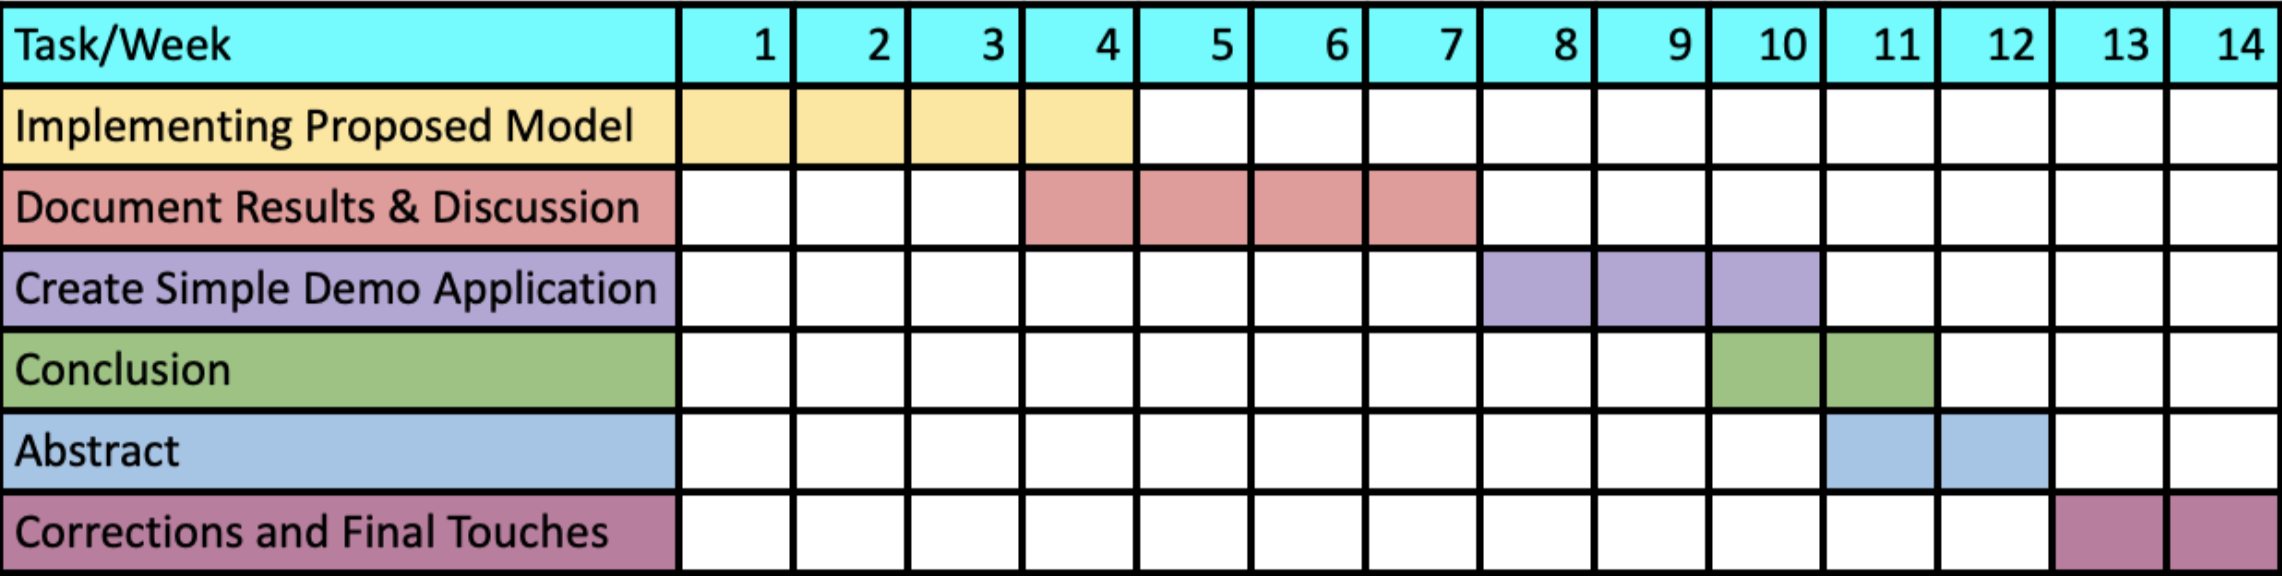
\includegraphics[width=0.5\linewidth]{FYP2-Gantt_Chart.png}
    \caption{Note. Figure depicts planned timeline for FYP2 for MMU Term 2610}
    \label{fig:FYP2-GANTT_CHART}
\end{figure}

\section{Conclusion}

\printbibliography

\end{document}